\chapter{Results}
This chapter presents the results of two \textbf{evaluation sessions conducted with two professional architects}, hereafter referred to as \textit{architect A} and \textit{architect B}. Each architect evaluated AI-generated images, which the researcher generated using different combinations of the architect's three LoRA models.\\~\\
To facilitate the sessions, the researcher prepared a selection of images in advance, as generating images requires some time. Additional images were generated during the sessions themselves, allowing the architect to interact with the image generation process and to observe outputs in real time.\\~\\
The chapter is divided in two sections; one for each architect. Within each section, the phases are explained in chronological order.
\newpage
\section{Architect A}
\subsection{Sketch design phase}
\subsubsection{Starting images}
\begin{figure}[H]
  \centering
  {\footnotesize
  \renewcommand{\arraystretch}{1.1}
  \setlength{\tabcolsep}{4pt}
  \begin{tabular}{c c c c c c c c}
    & \shortstack{\textbf{Stamp-}\\\textbf{beton}} 
    & \shortstack{\textbf{3D-}\\\textbf{effect}} 
    & \textbf{Geleding} 
    & \shortstack{\textbf{Stampbeton}\\ \textbf{\& 3D-effect}} 
    & \shortstack{\textbf{Stampbeton}\\ \textbf{\& Geleding}} 
    & \shortstack{\textbf{3D-effect} \&\\ \textbf{Geleding}} 
    & \shortstack{\textbf{Stampbeton,}\\\textbf{3D-effect \&}\\\textbf{Geleding}} \\

    \shortstack{\textbf{With}\\\textbf{LoRA}} & \href{https://github.com/matijspeeters/Thesis_Lora/blob/main/Results/Architect%20A/Sketch%20design/Met_lora_00001_.png}{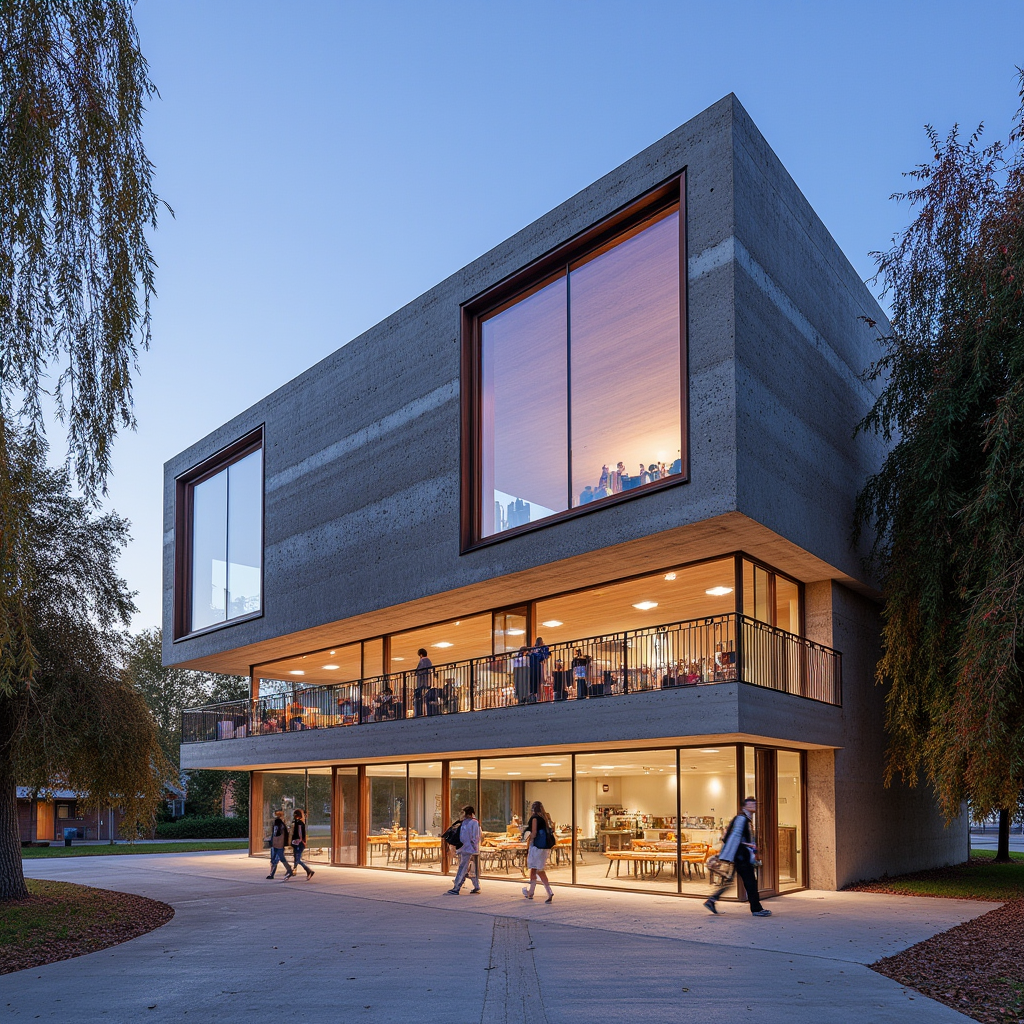
\includegraphics[width=0.12\textwidth]{Images/Results/Architect-A_Fixed-images/1-sketch_design/Met_lora_00001_.png}} & \href{https://github.com/matijspeeters/Thesis_Lora/blob/main/Results/Architect%20A/Sketch%20design/Met_lora_00002_.png}{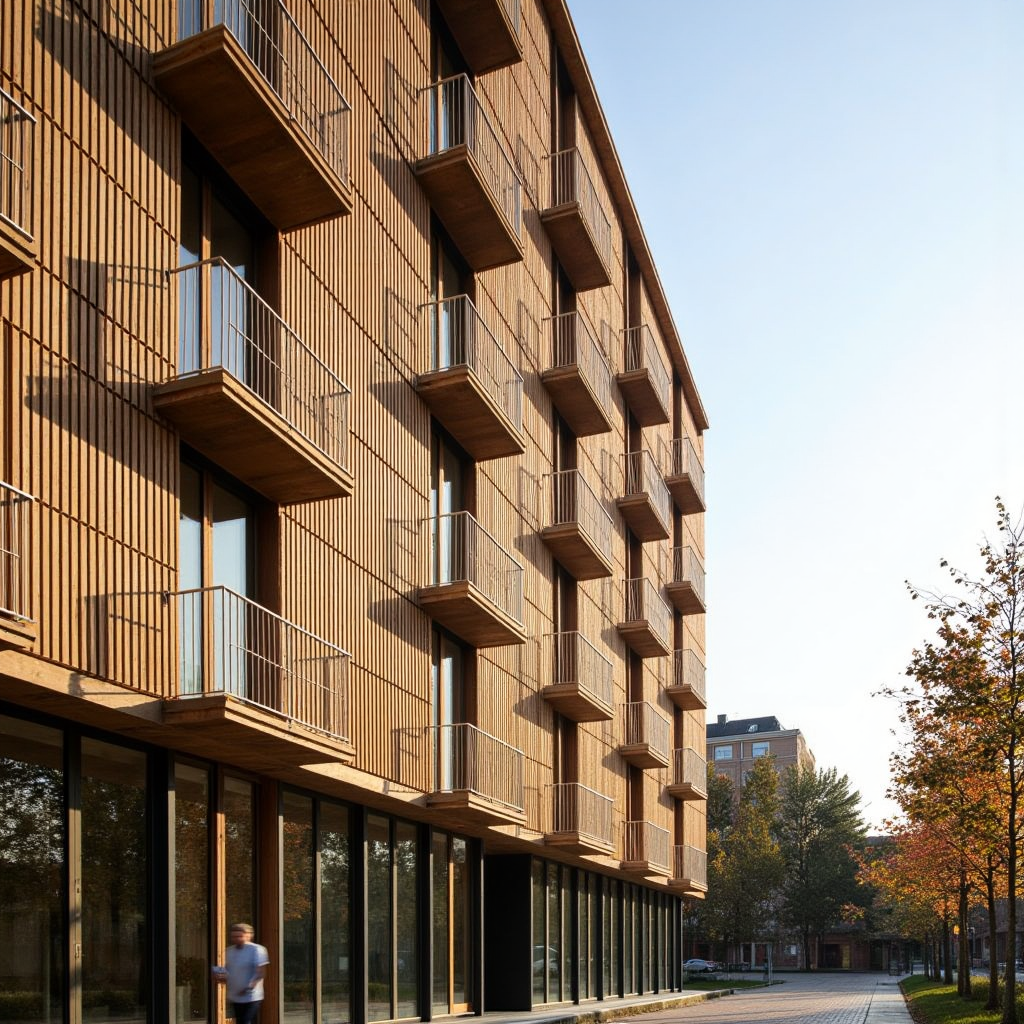
\includegraphics[width=0.12\textwidth]{Images/Results/Architect-A_Fixed-images/1-sketch_design/Met_lora_00002_.png}} &
    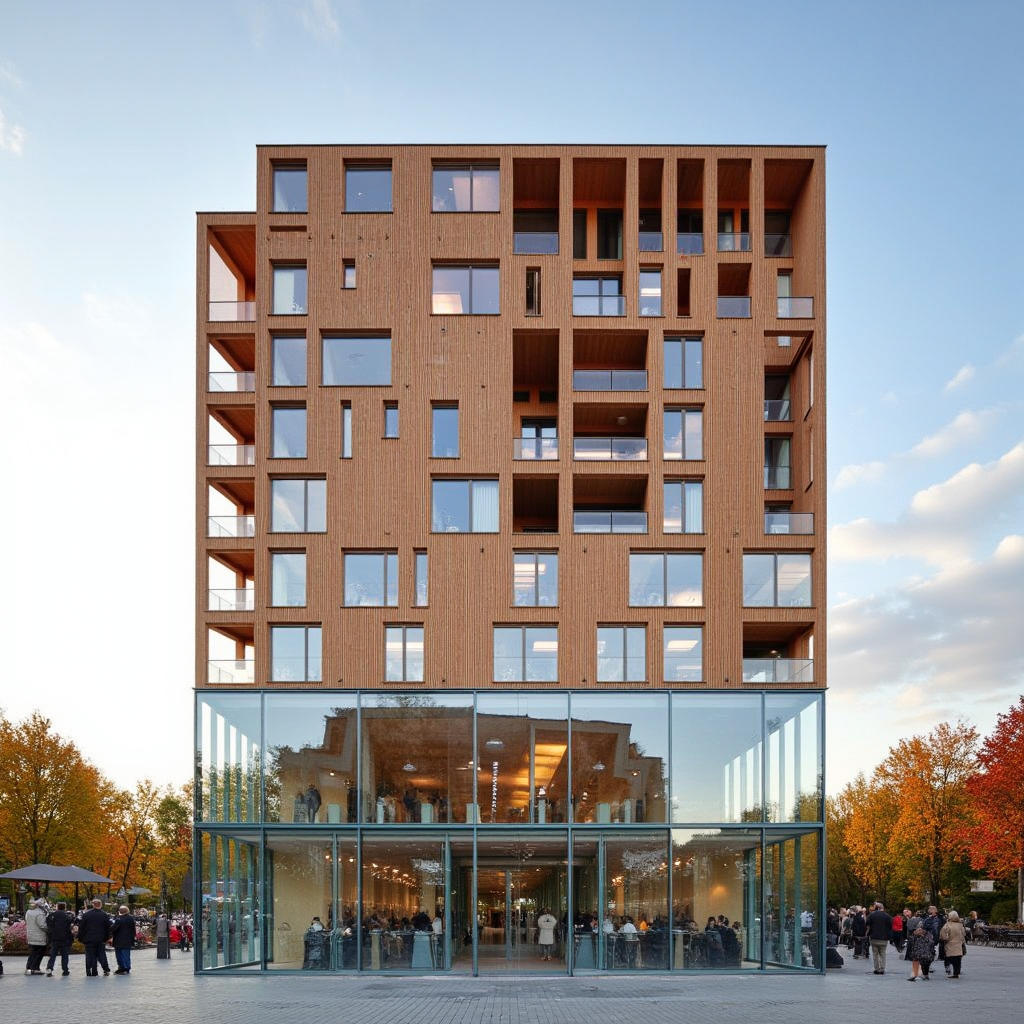
\includegraphics[width=0.12\textwidth]{Images/Results/Architect-A_Fixed-images/1-sketch_design/Met_lora_00017_ (2).png} &
    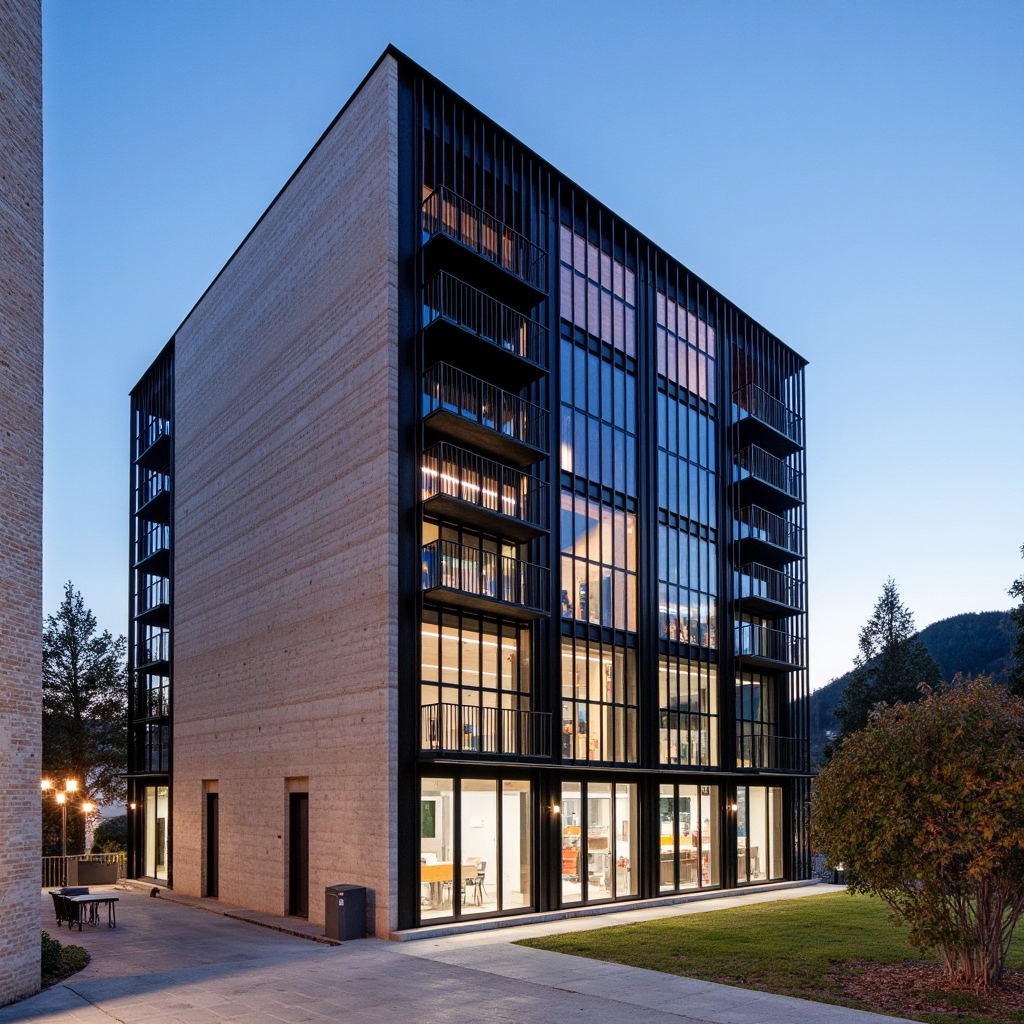
\includegraphics[width=0.12\textwidth]{Images/Results/Architect-A_Fixed-images/1-sketch_design/Met_lora_00029_.png} &
    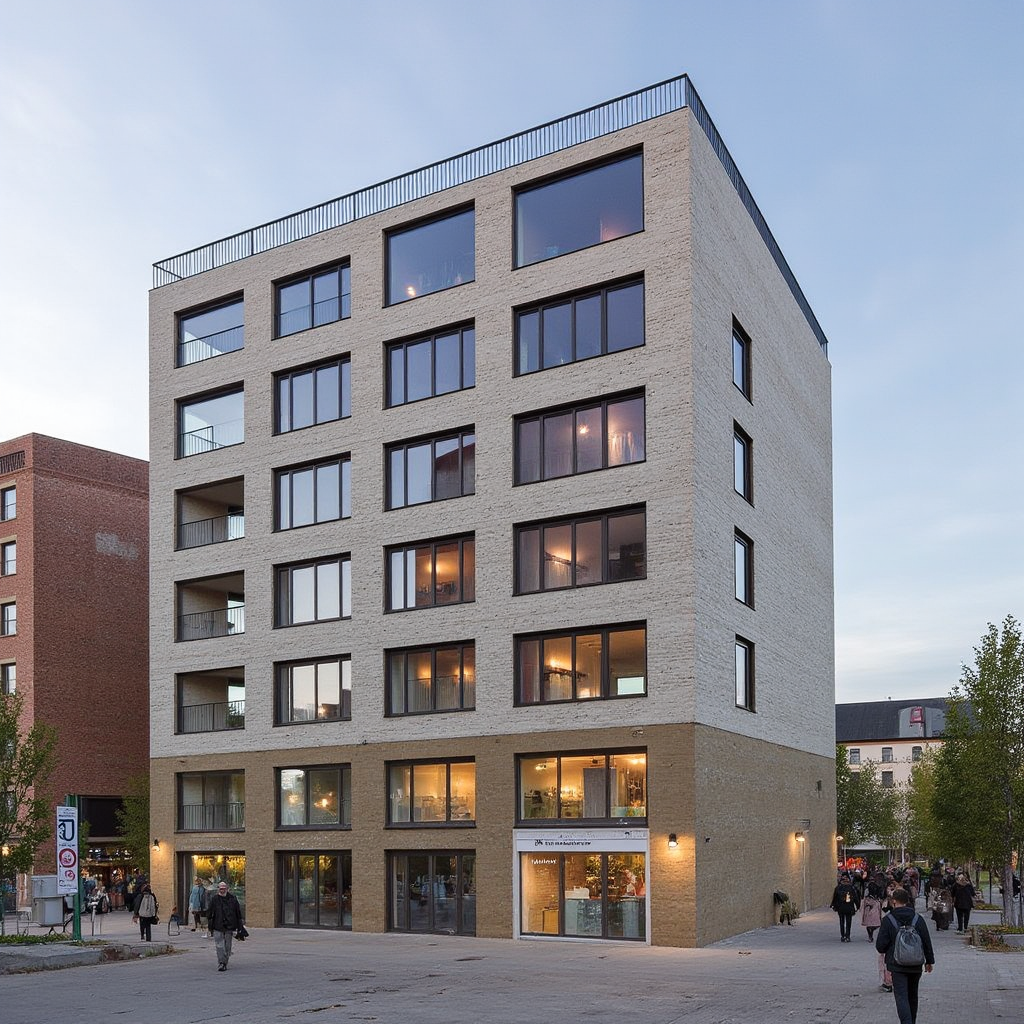
\includegraphics[width=0.12\textwidth]{Images/Results/Architect-A_Fixed-images/1-sketch_design/Met_lora_00039_.png} &
    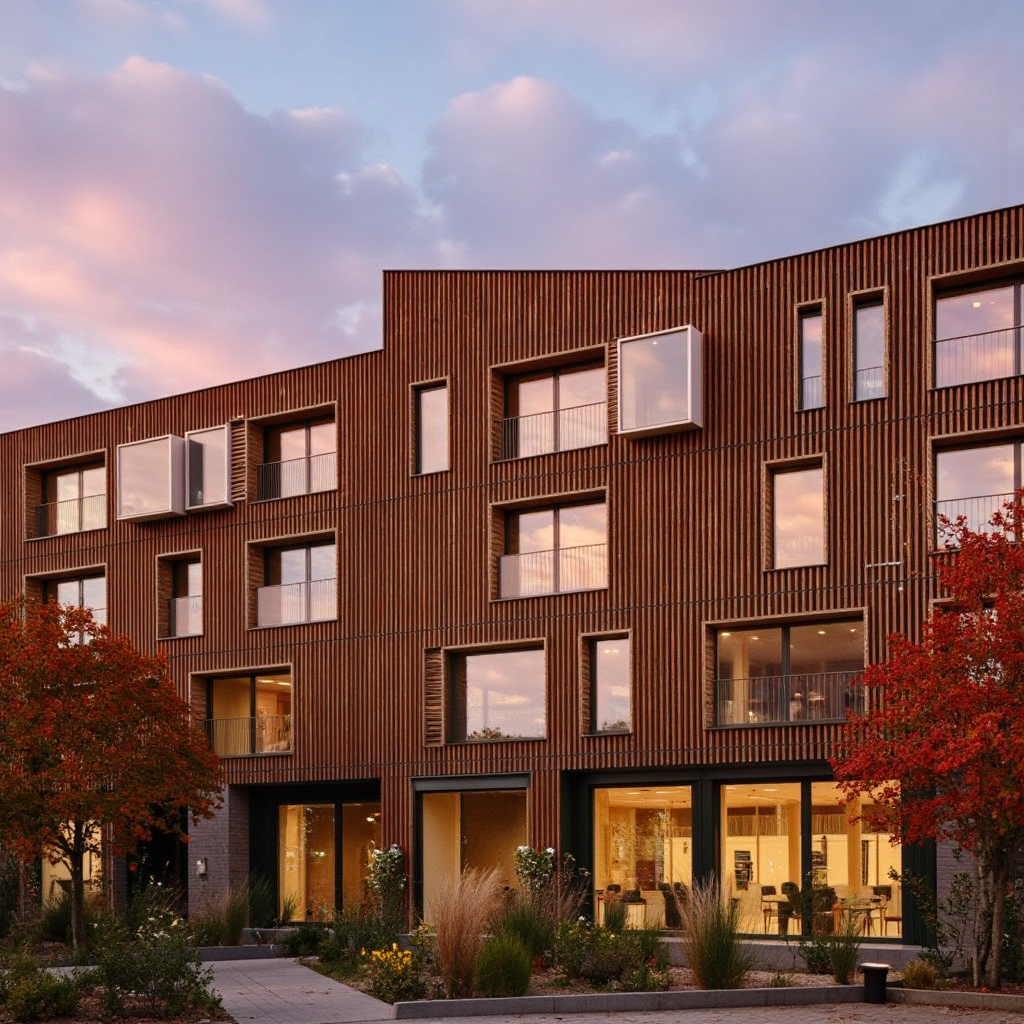
\includegraphics[width=0.12\textwidth]{Images/Results/Architect-A_Fixed-images/1-sketch_design/Met_lora_00043_ (1).png} &
    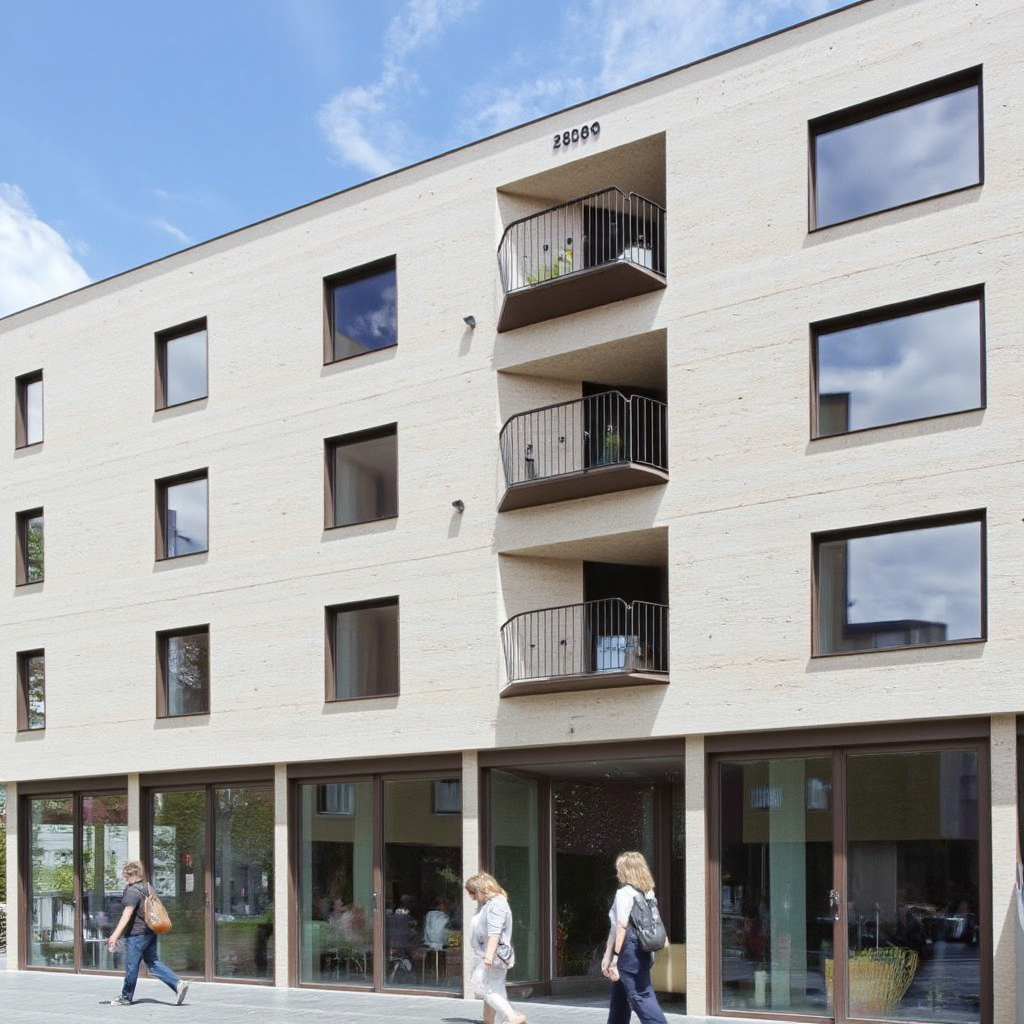
\includegraphics[width=0.12\textwidth]{Images/Results/Architect-A_Fixed-images/1-sketch_design/Met_lora_00058_.png} \\

    \shortstack{\textbf{Without}\\\textbf{LoRA}} &
    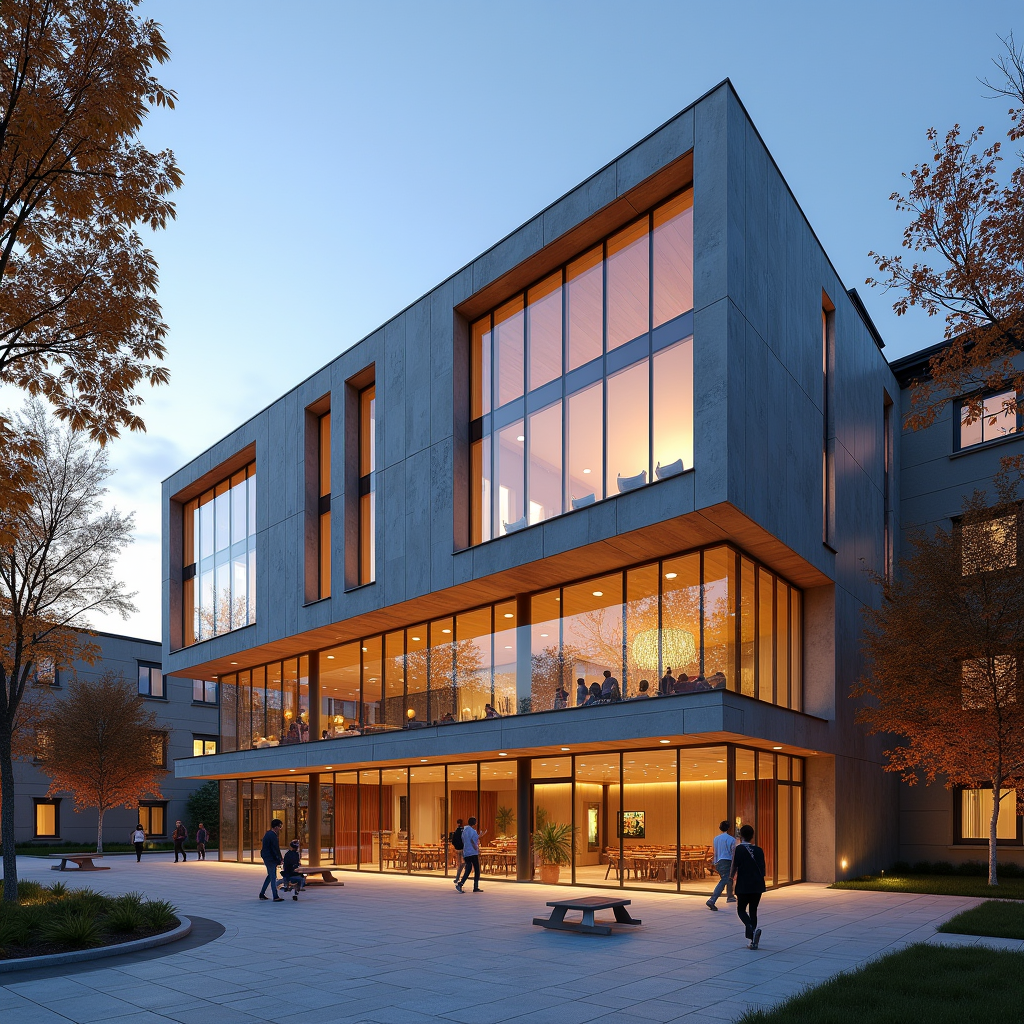
\includegraphics[width=0.12\textwidth]{Images/Results/Architect-A_Fixed-images/1-sketch_design/Zonder_lora_00001_.png} &
    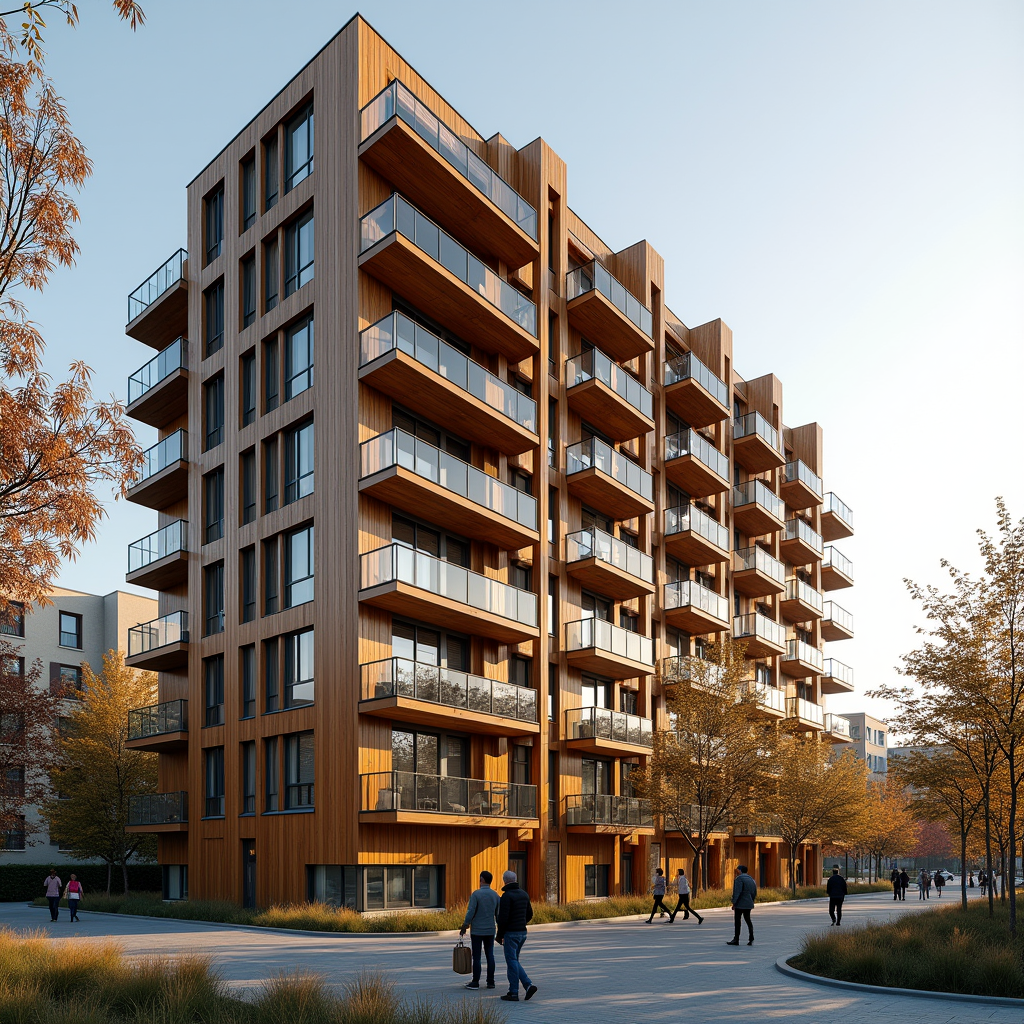
\includegraphics[width=0.12\textwidth]{Images/Results/Architect-A_Fixed-images/1-sketch_design/Zonder_lora_00002_.png} &
    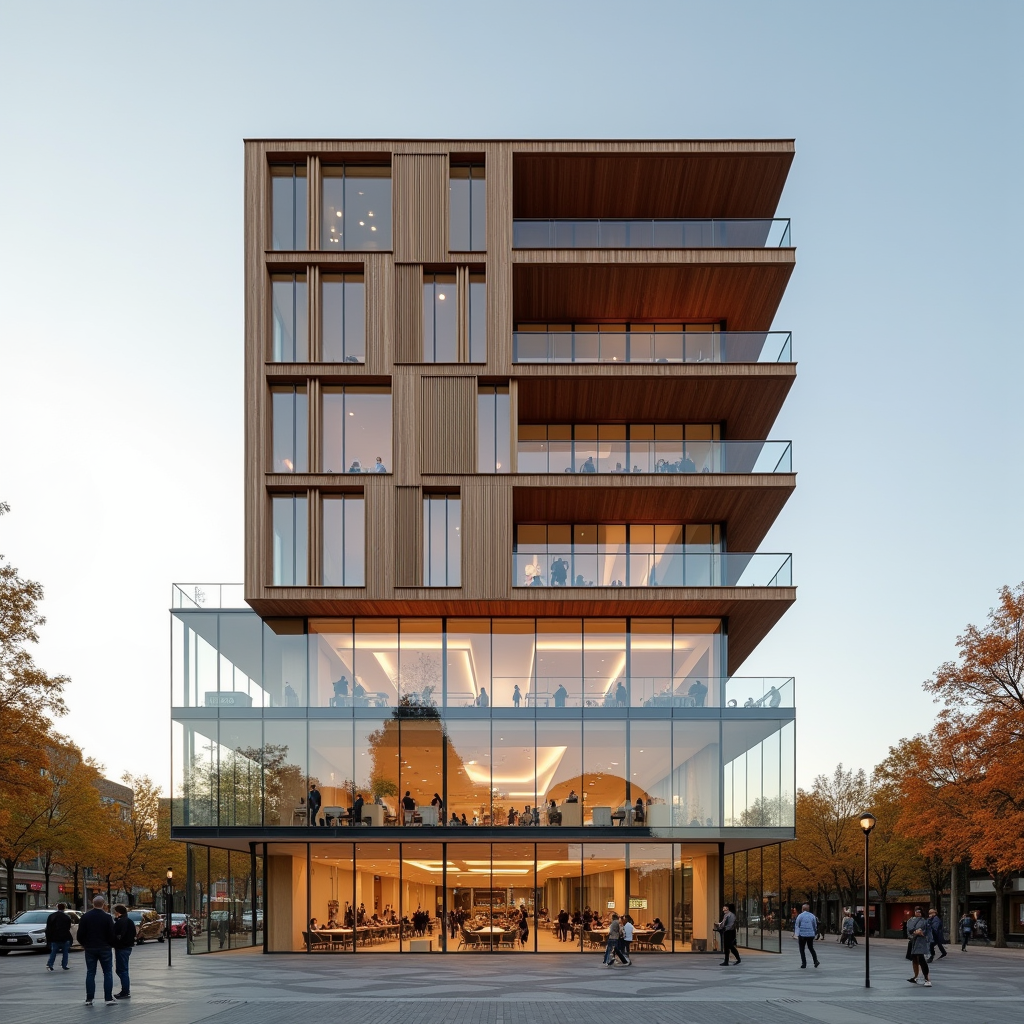
\includegraphics[width=0.12\textwidth]{Images/Results/Architect-A_Fixed-images/1-sketch_design/Zonder_lora_00017_ (1).png} &
    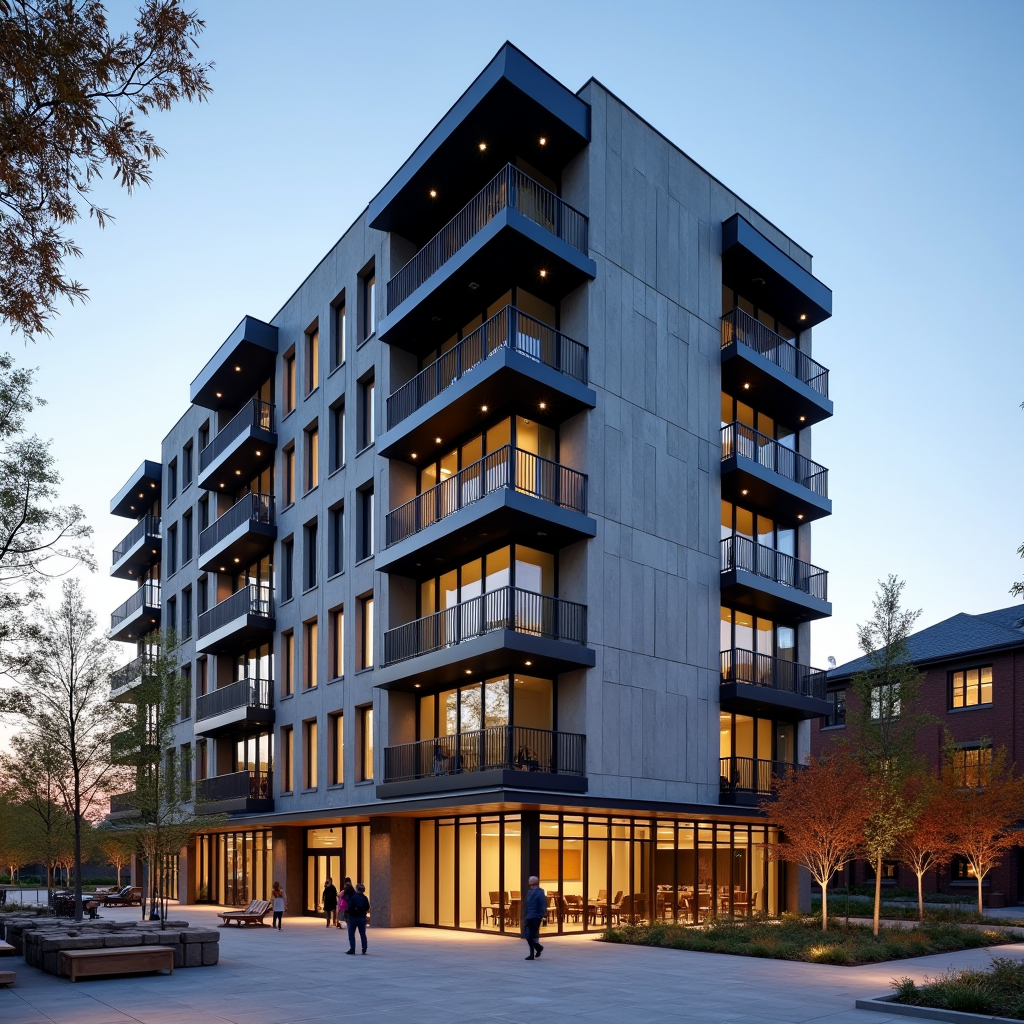
\includegraphics[width=0.12\textwidth]{Images/Results/Architect-A_Fixed-images/1-sketch_design/Zonder_lora_00029_.png} &
    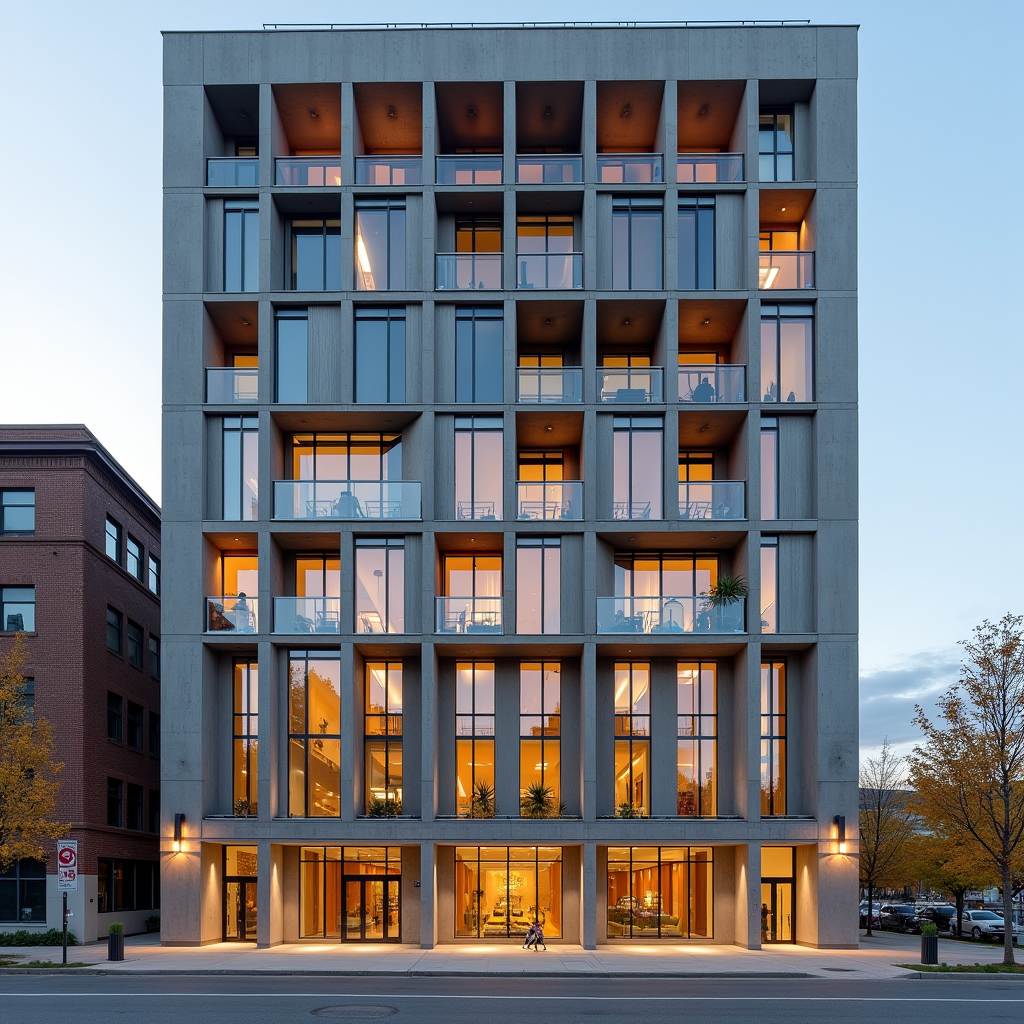
\includegraphics[width=0.12\textwidth]{Images/Results/Architect-A_Fixed-images/1-sketch_design/Zonder_lora_00039_.png} &
    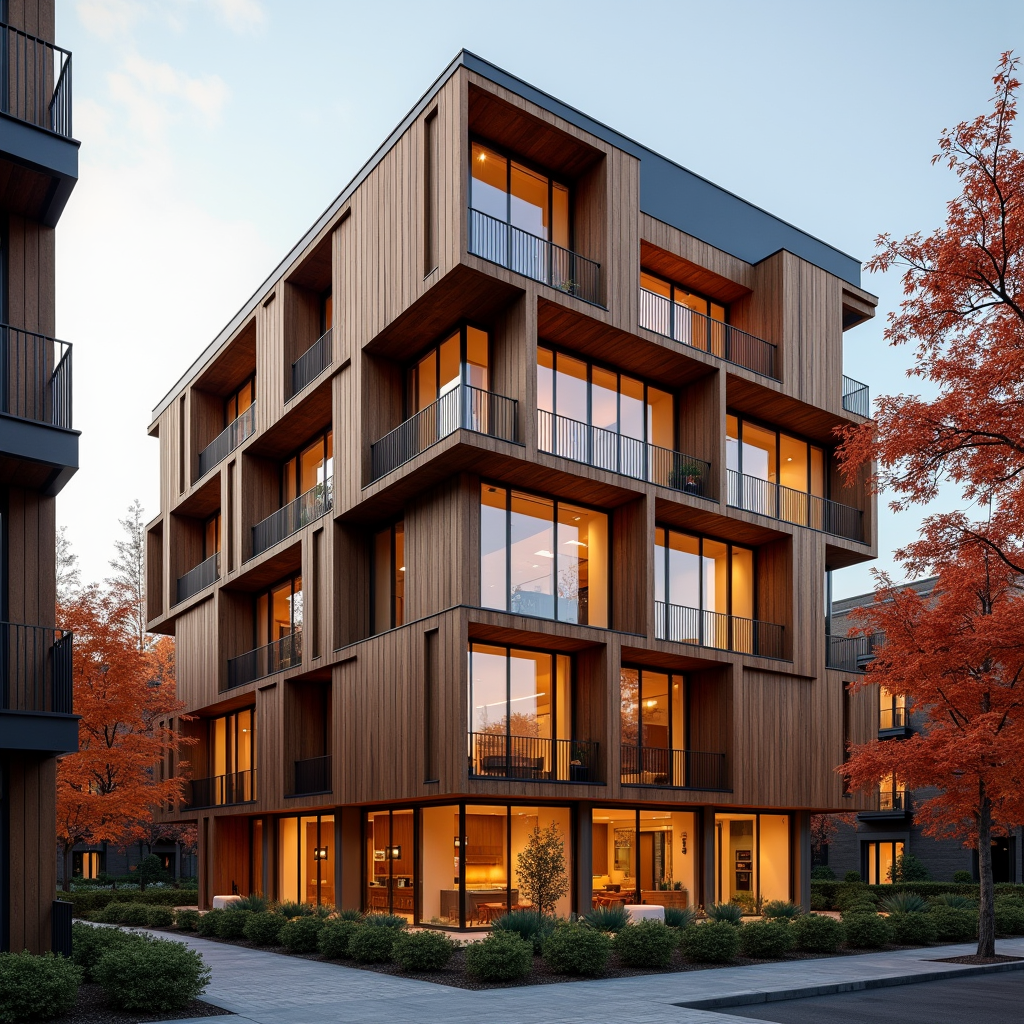
\includegraphics[width=0.12\textwidth]{Images/Results/Architect-A_Fixed-images/1-sketch_design/Zonder_lora_00043_ (1).png} &
    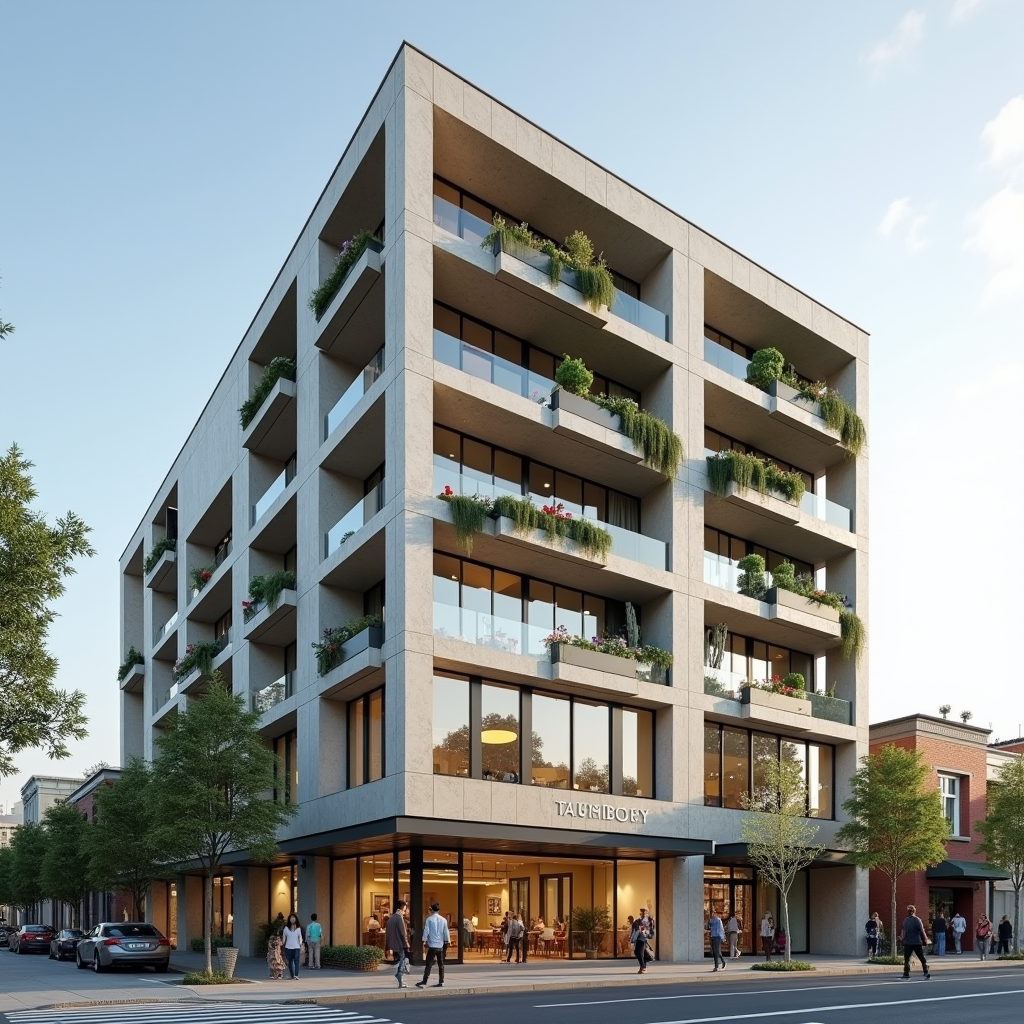
\includegraphics[width=0.12\textwidth]{Images/Results/Architect-A_Fixed-images/1-sketch_design/Zonder_lora_00058_.png} \\
  \end{tabular}
  }
  \caption{Starting images in the sketch design phase of architect A.}
  \label{fig:horizontal-lora-comparison}
\end{figure}
\subsubsection{Selected starting image}
Architect A selected the image in figure \ref{fig:A-sketch-selected}, which was generated with the \textbf{3D-effect} and \textbf{Geleding} models. His reasons were two-fold: the 'warm facade cladding' and 'a clear connection to the ground level'.
\begin{figure}[H]
    \centering
    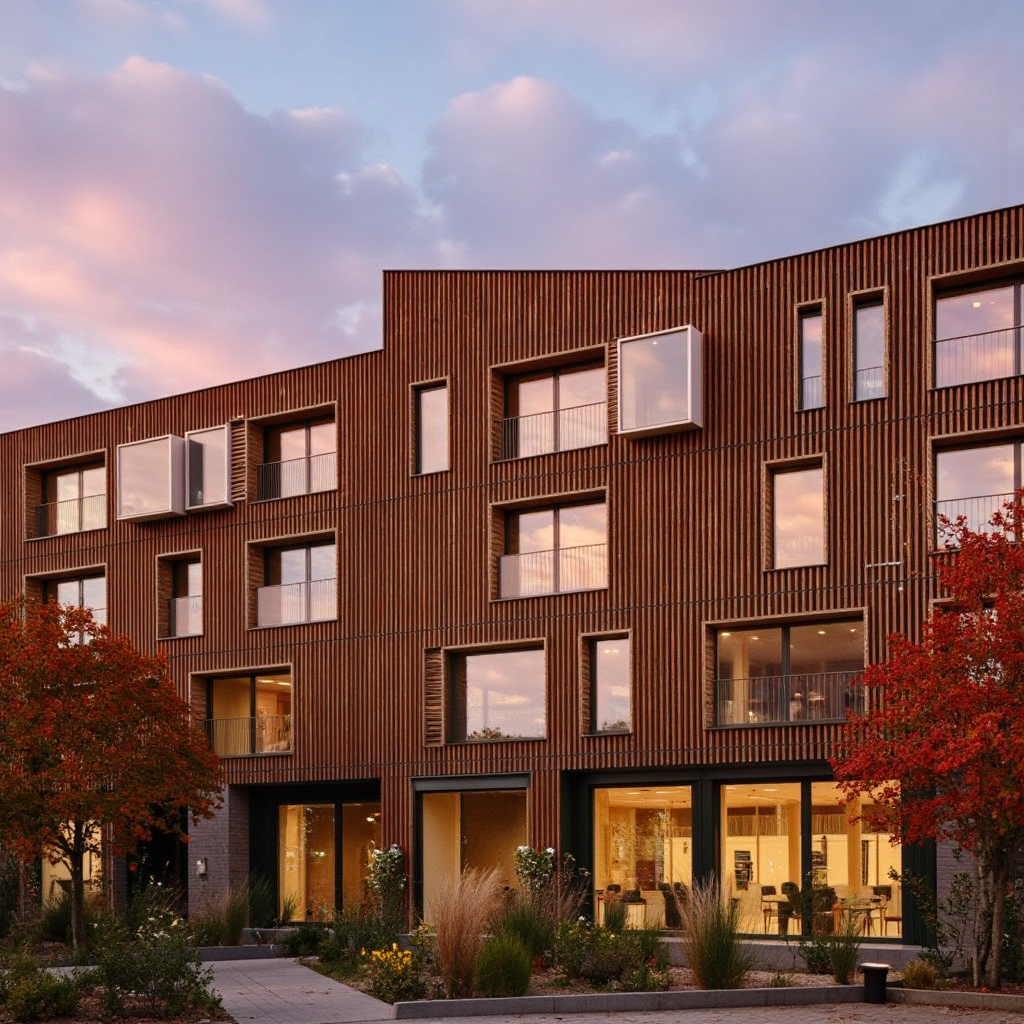
\includegraphics[width=0.3\linewidth]{Images/Results/Architect-A_Fixed-images/1-sketch_design/Met_lora_00043_ (1).png}
    \caption{Architect A's selected starting image for the sketch design phase.}
    \label{fig:A-sketch-selected}
\end{figure}
\subsubsection{Preferred generated images}
Architect A selected 3 preferred images (figure \ref{fig:A-sketch-favourite}) among the generated images during the sketch design phase. In his opinion, image 1 and 2 shared a 'combination of old and new'. The building in image 3 was 'playing with volumes, rather than referring to something'. It 'introduces a very strong gesture' and 'interacts with nature'.
\begin{figure}[H]
    \centering
    \begin{tabular}{ccc}
         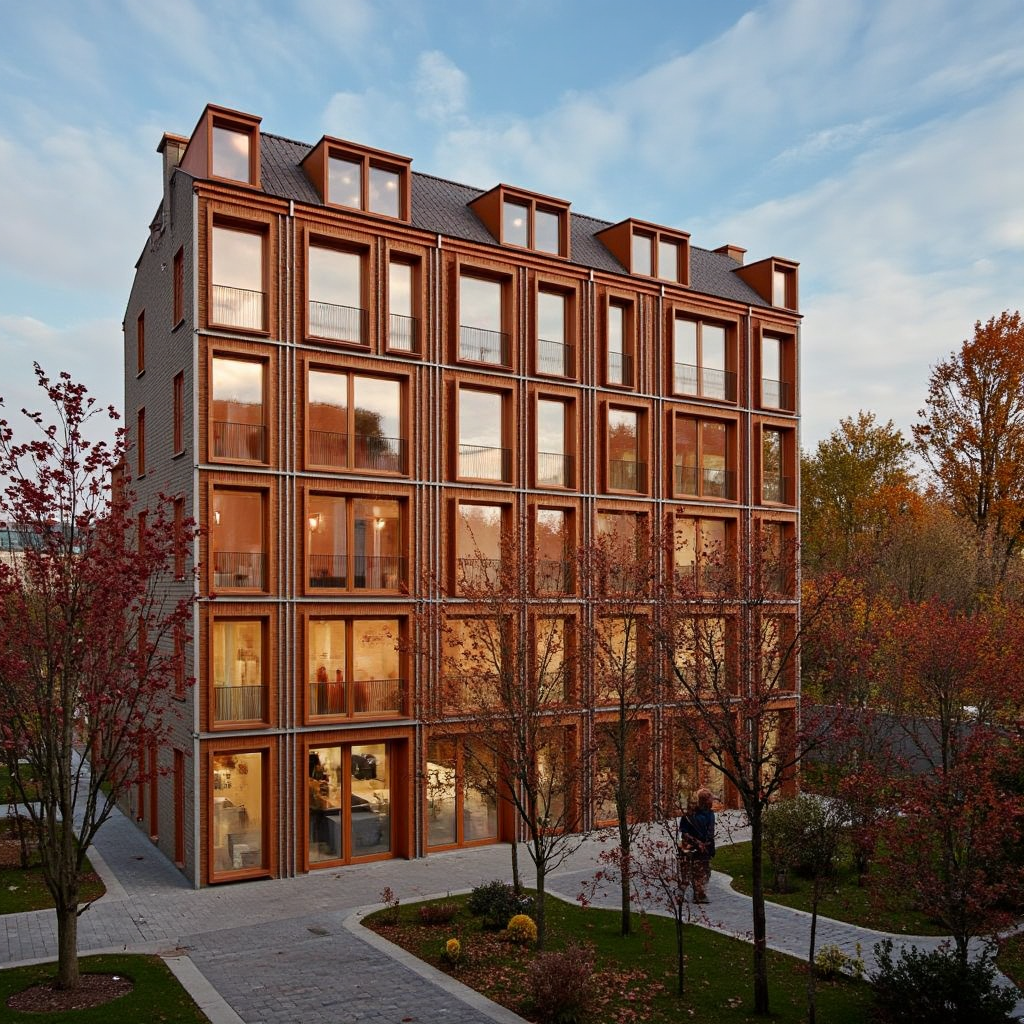
\includegraphics[width=0.3\linewidth]{Images/Results/Architect A/1. sketch phase/Met_lora_00126_.png}
         & 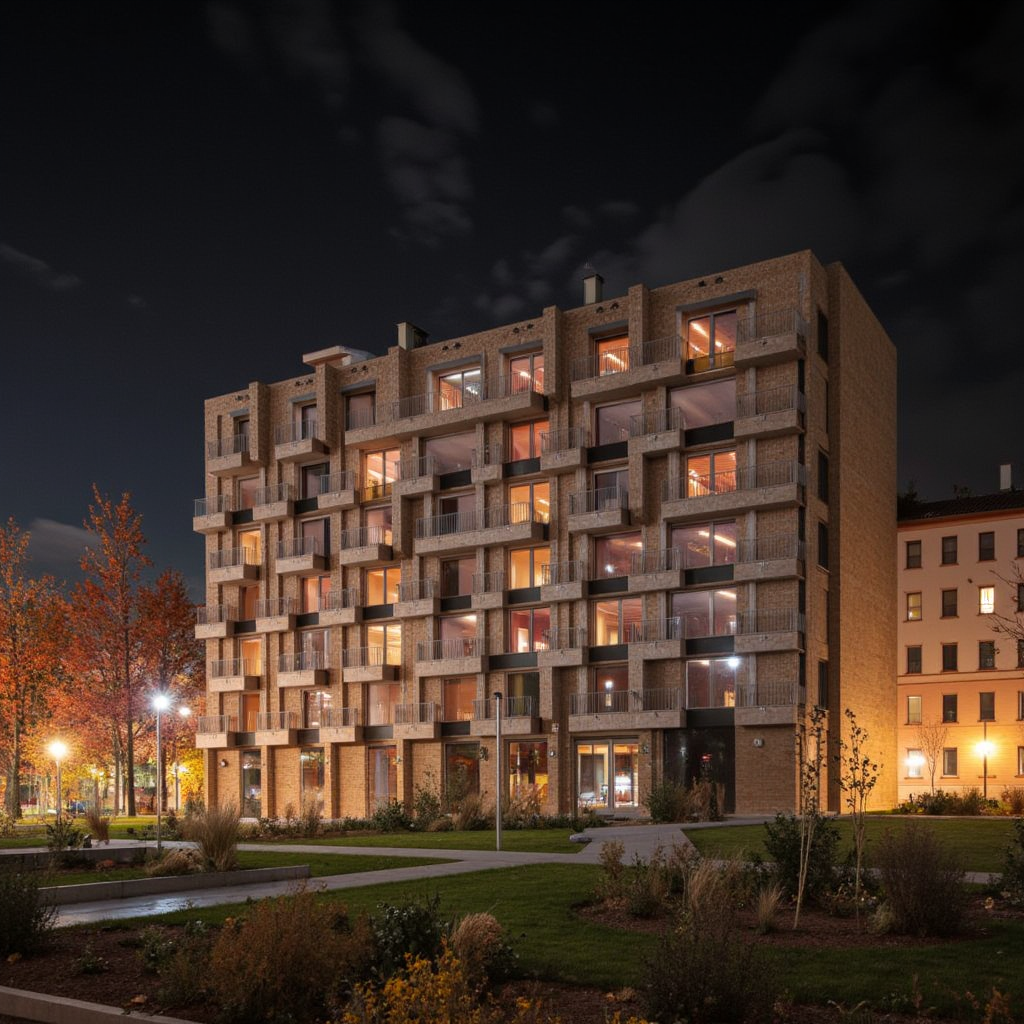
\includegraphics[width=0.3\linewidth]{Images/Results/Architect A/1. sketch phase/Met_lora_00139_.png}
         & 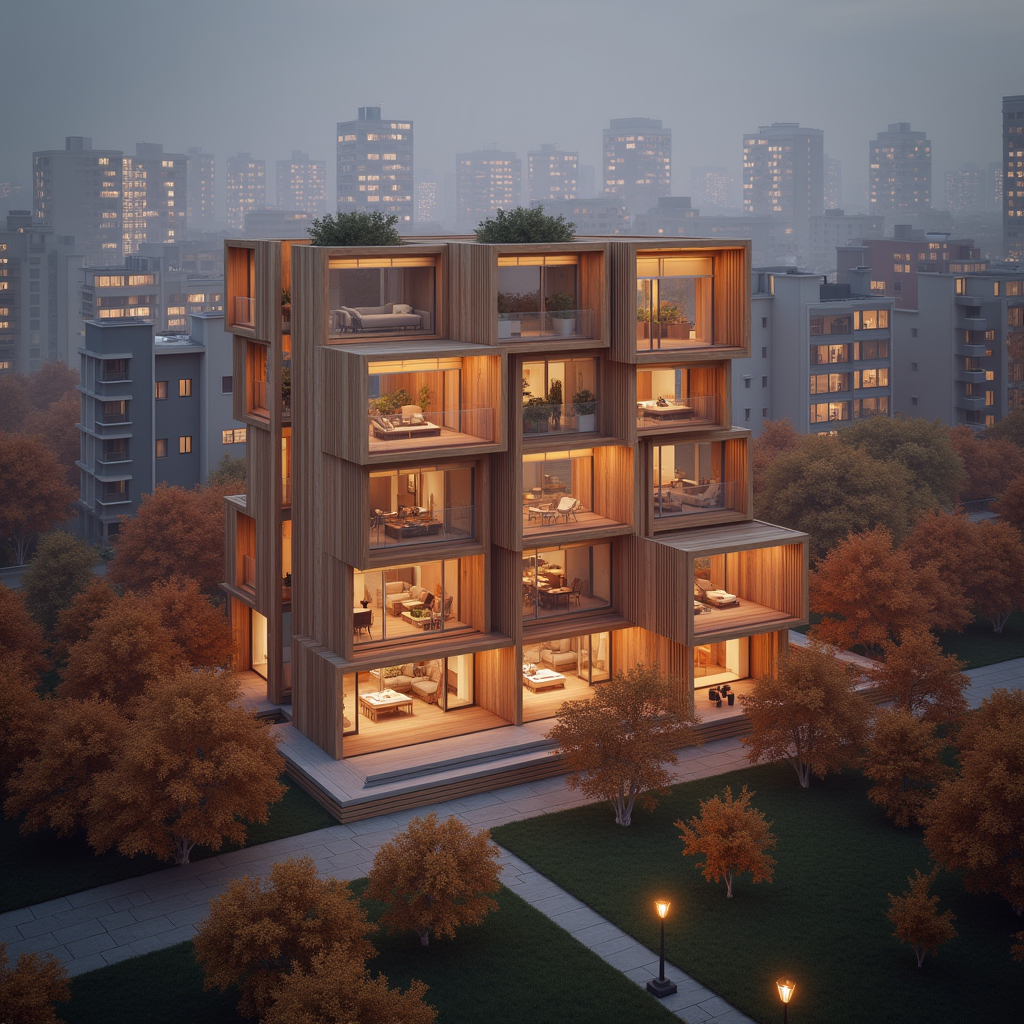
\includegraphics[width=0.3\linewidth]{Images/Results/Architect A/1. sketch phase/Zonder_lora_00144_.png}\\
         \textit{(1)} & \textit{(2)} & \textit{(3)}
    \end{tabular}
    \caption{Architect A's favourite images in the sketch design phase.}
    \label{fig:A-sketch-favourite}
\end{figure}
\subsection{Preliminary design phase}
\subsubsection{Starting images}
\begin{figure}[H]
  \centering
  {\footnotesize
  \renewcommand{\arraystretch}{1.1}
  \setlength{\tabcolsep}{4pt}
  \begin{tabular}{c c c c c c c c}
    & \shortstack{\textbf{Stamp-}\\\textbf{beton}} 
    & \shortstack{\textbf{3D-}\\\textbf{effect}} 
    & \textbf{Geleding} 
    & \shortstack{\textbf{Stampbeton}\\ \textbf{\& 3D-effect}} 
    & \shortstack{\textbf{Stampbeton}\\ \textbf{\& Geleding}} 
    & \shortstack{\textbf{3D-effect} \&\\ \textbf{Geleding}} 
    & \shortstack{\textbf{Stampbeton,}\\\textbf{3D-effect \&}\\\textbf{Geleding}} \\

    \shortstack{\textbf{With}\\\textbf{LoRA}} & 
    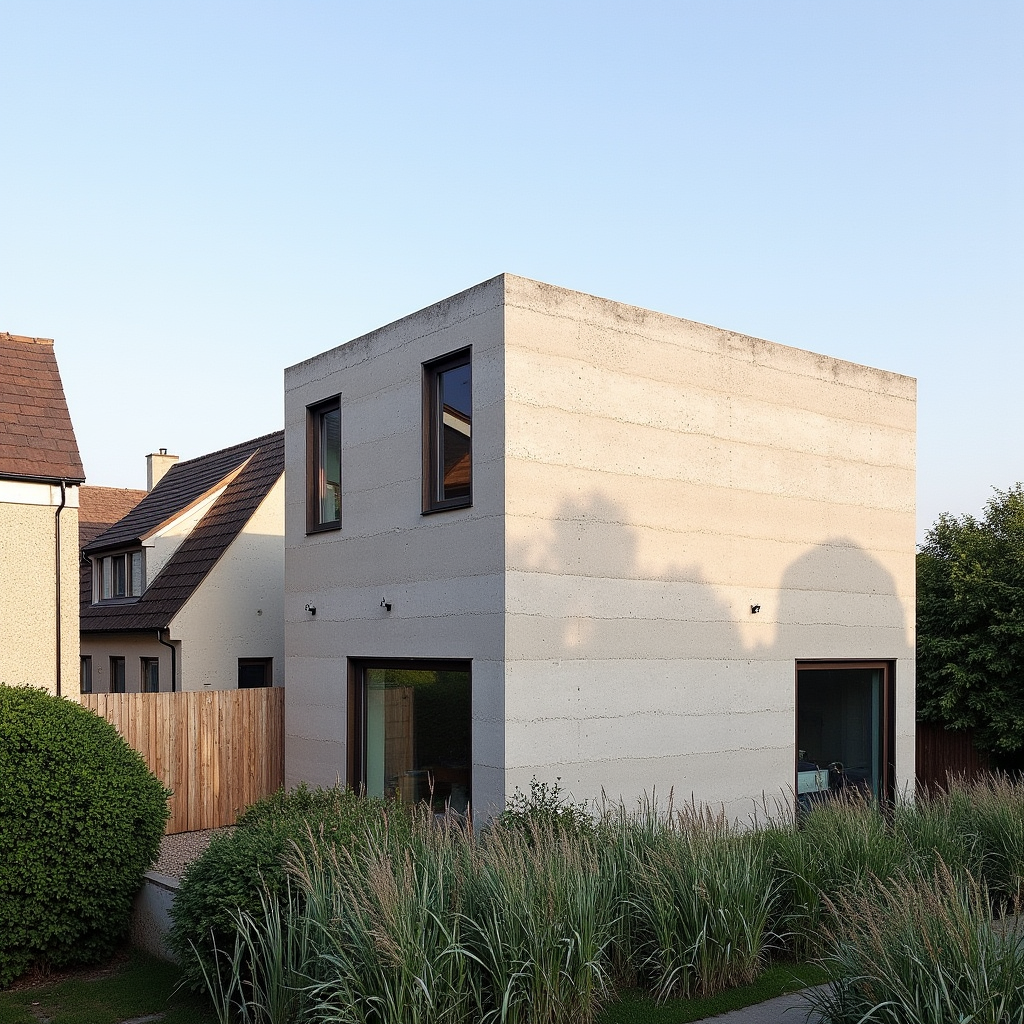
\includegraphics[width=0.12\textwidth]{Images/Results/Architect-A_Fixed-images/2-preliminary_design/Met_lora_00059_ (1).png} & 
    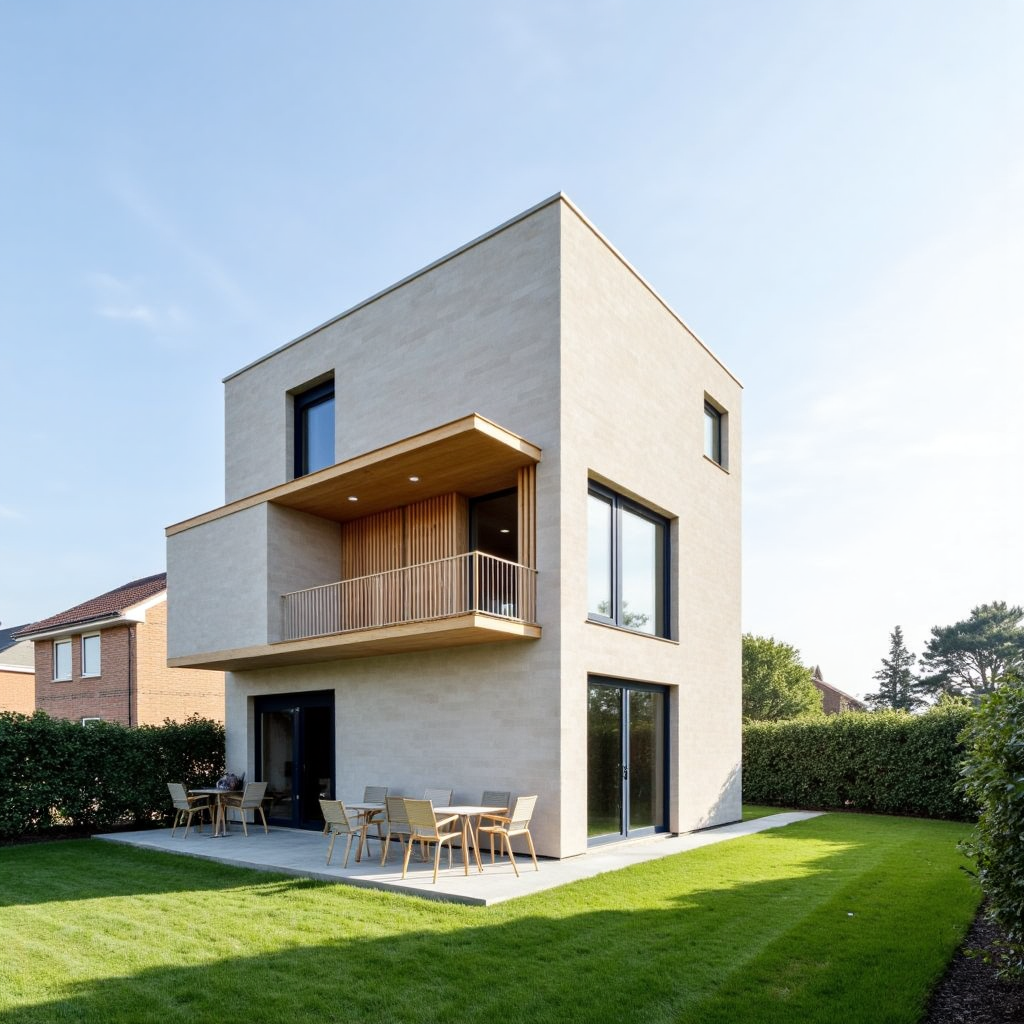
\includegraphics[width=0.12\textwidth]{Images/Results/Architect-A_Fixed-images/2-preliminary_design/Met_lora_00061_.png} &
    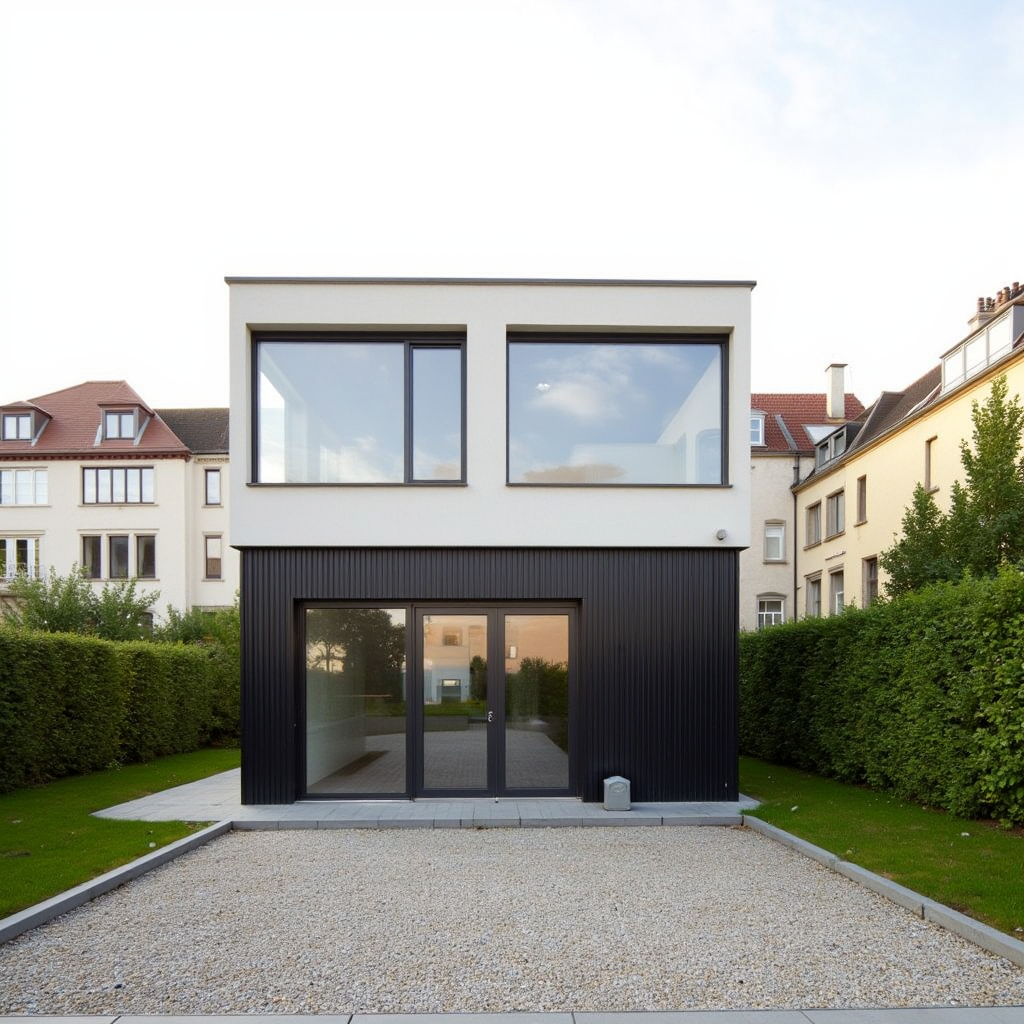
\includegraphics[width=0.12\textwidth]{Images/Results/Architect-A_Fixed-images/2-preliminary_design/Met_lora_00069_ (1).png} &
    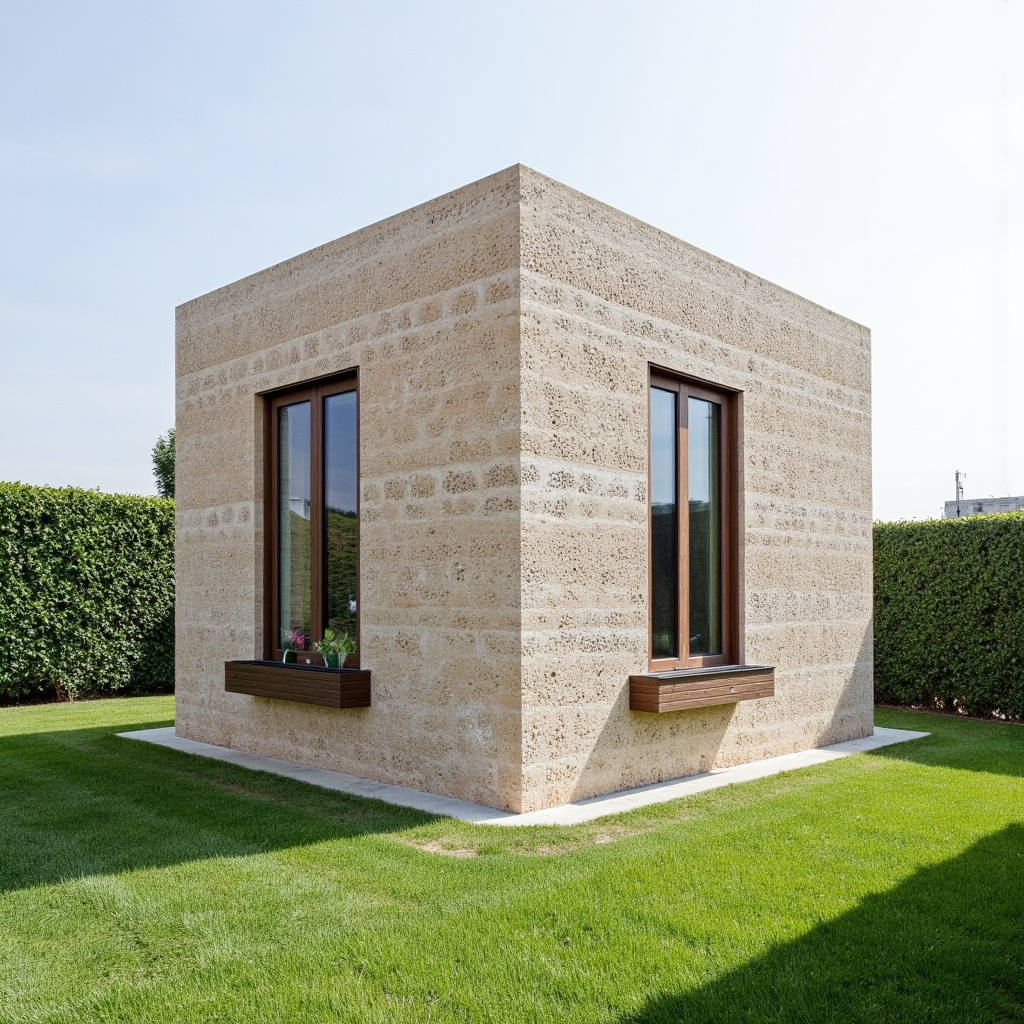
\includegraphics[width=0.12\textwidth]{Images/Results/Architect-A_Fixed-images/2-preliminary_design/Met_lora_00080_.png} &
    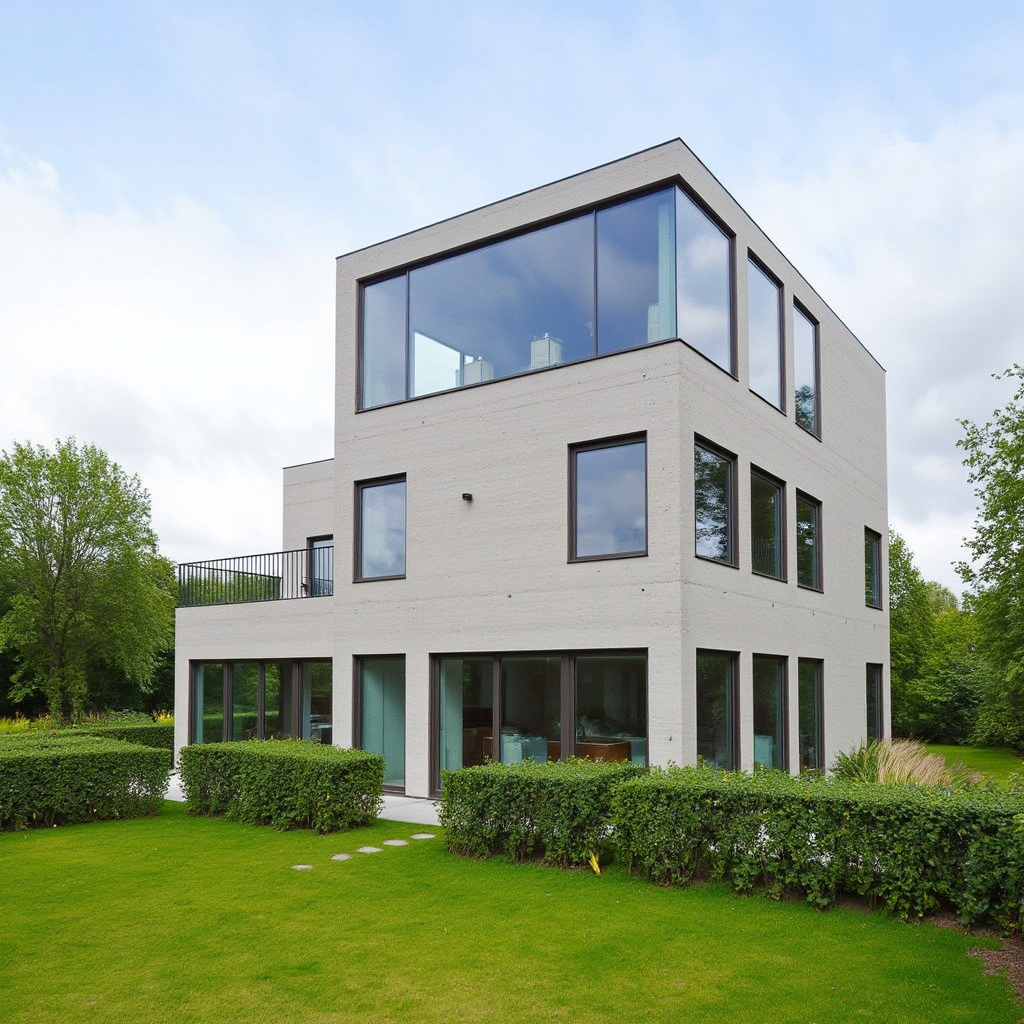
\includegraphics[width=0.12\textwidth]{Images/Results/Architect-A_Fixed-images/2-preliminary_design/Met_lora_00089_.png} &
    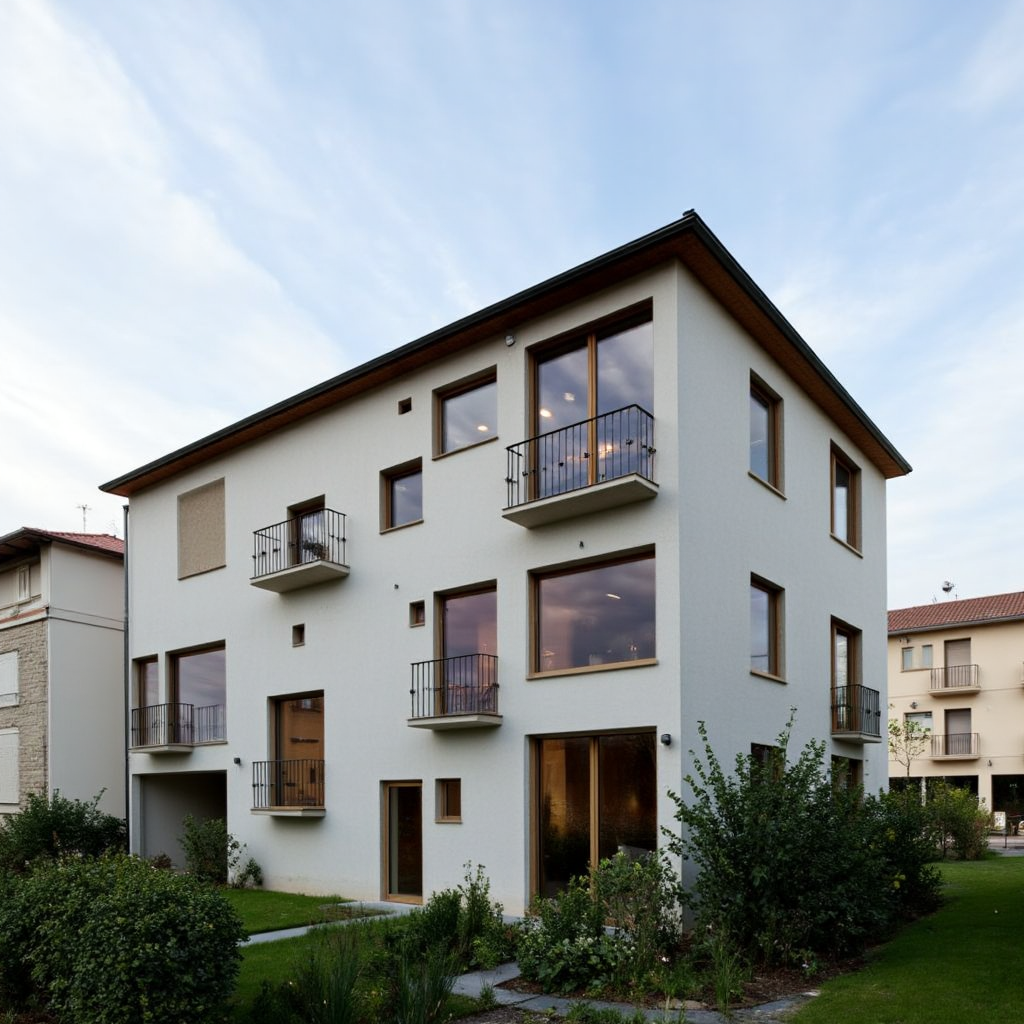
\includegraphics[width=0.12\textwidth]{Images/Results/Architect-A_Fixed-images/2-preliminary_design/Met_lora_00091_.png} &
    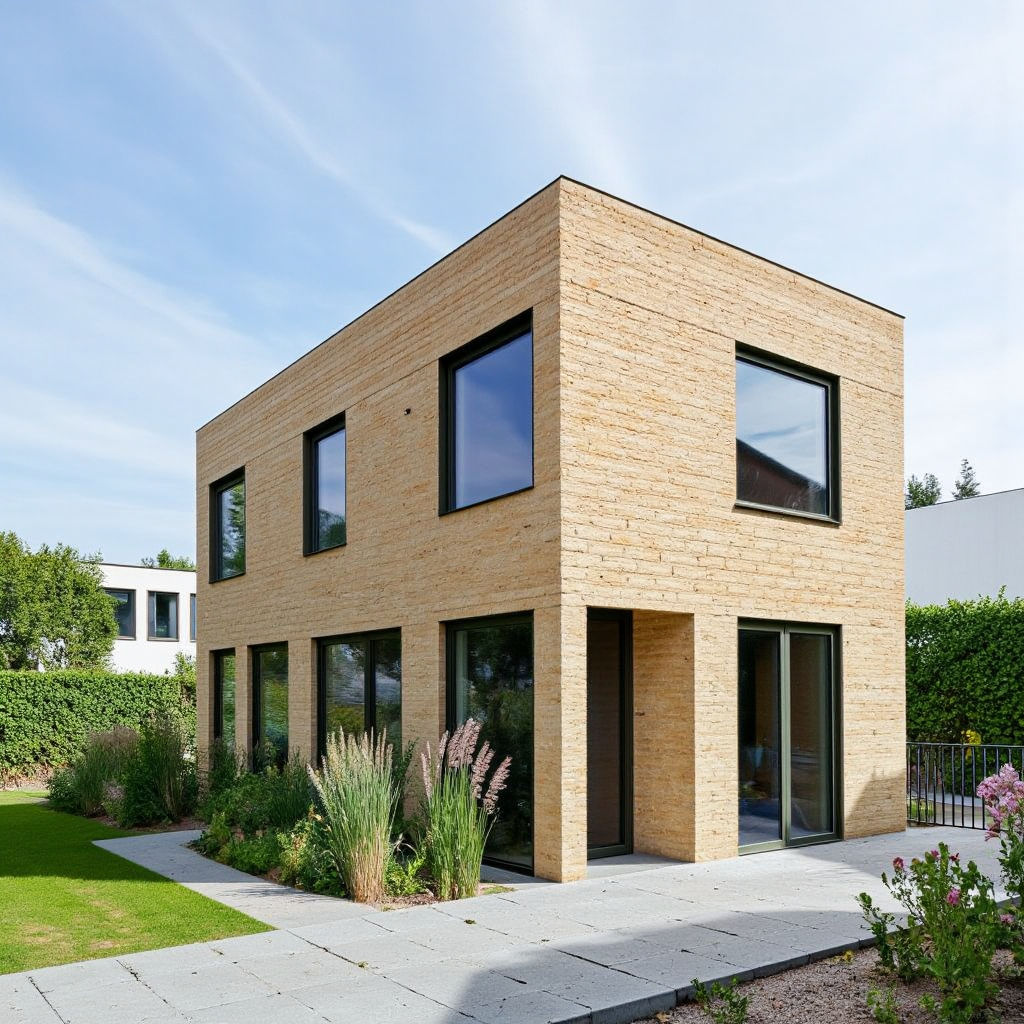
\includegraphics[width=0.12\textwidth]{Images/Results/Architect-A_Fixed-images/2-preliminary_design/Met_lora_00095_.png} \\

    \shortstack{\textbf{Without}\\\textbf{LoRA}} &
    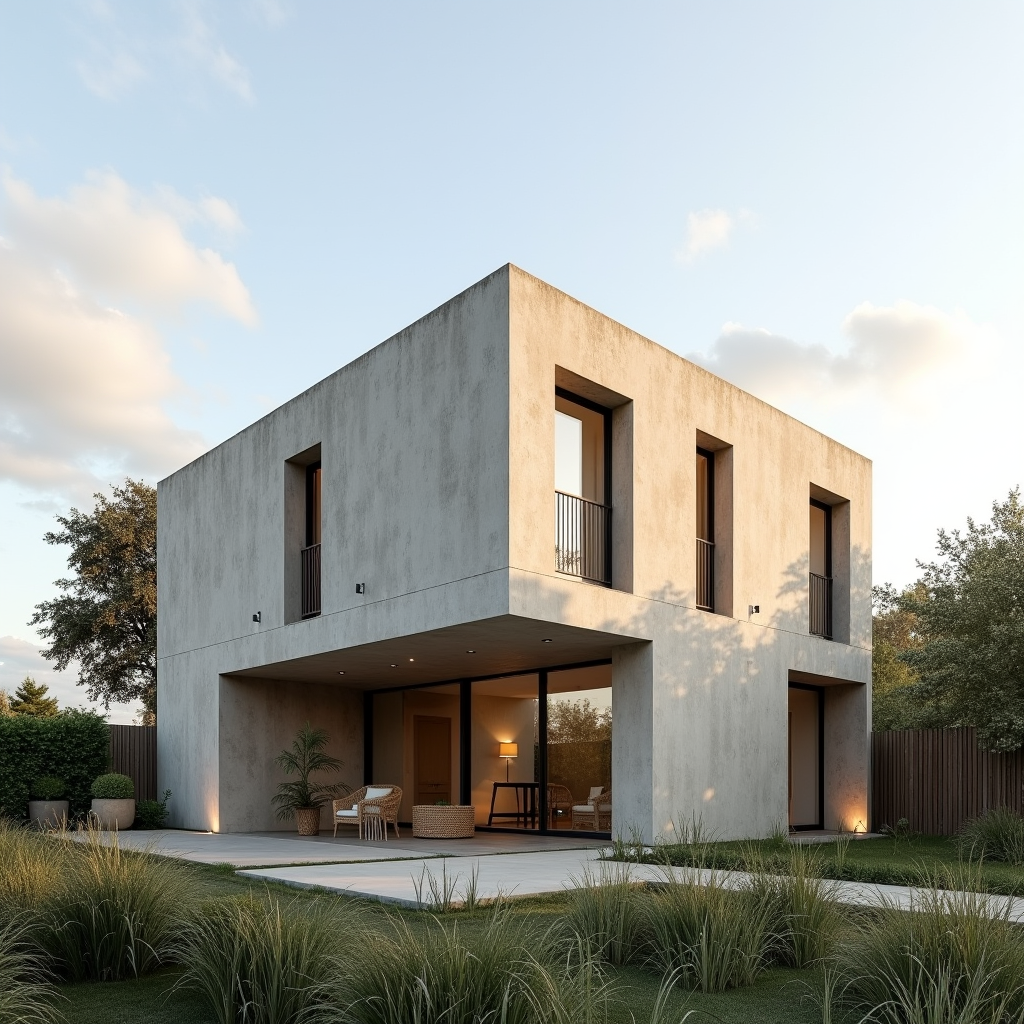
\includegraphics[width=0.12\textwidth]{Images/Results/Architect-A_Fixed-images/2-preliminary_design/Zonder_lora_00059_ (1).png} &
    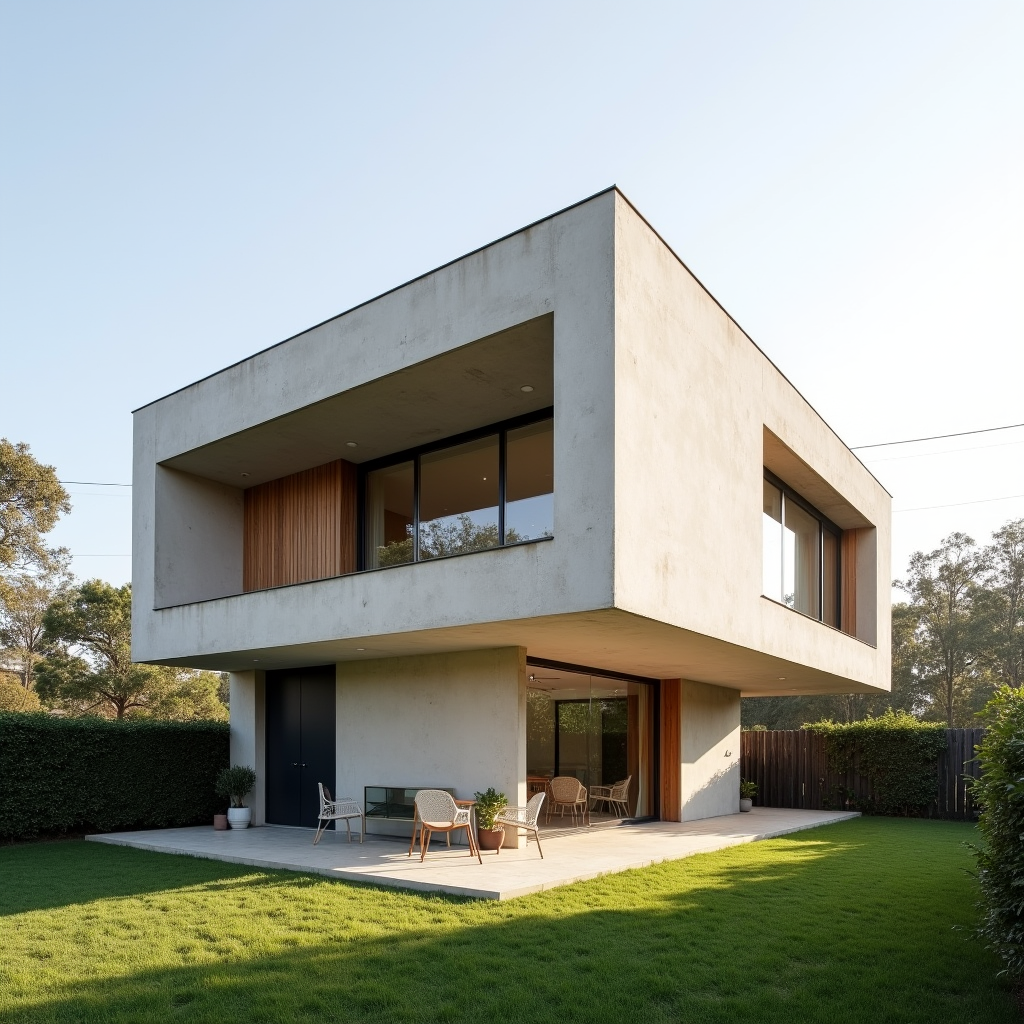
\includegraphics[width=0.12\textwidth]{Images/Results/Architect-A_Fixed-images/2-preliminary_design/Zonder_lora_00061_.png} &
    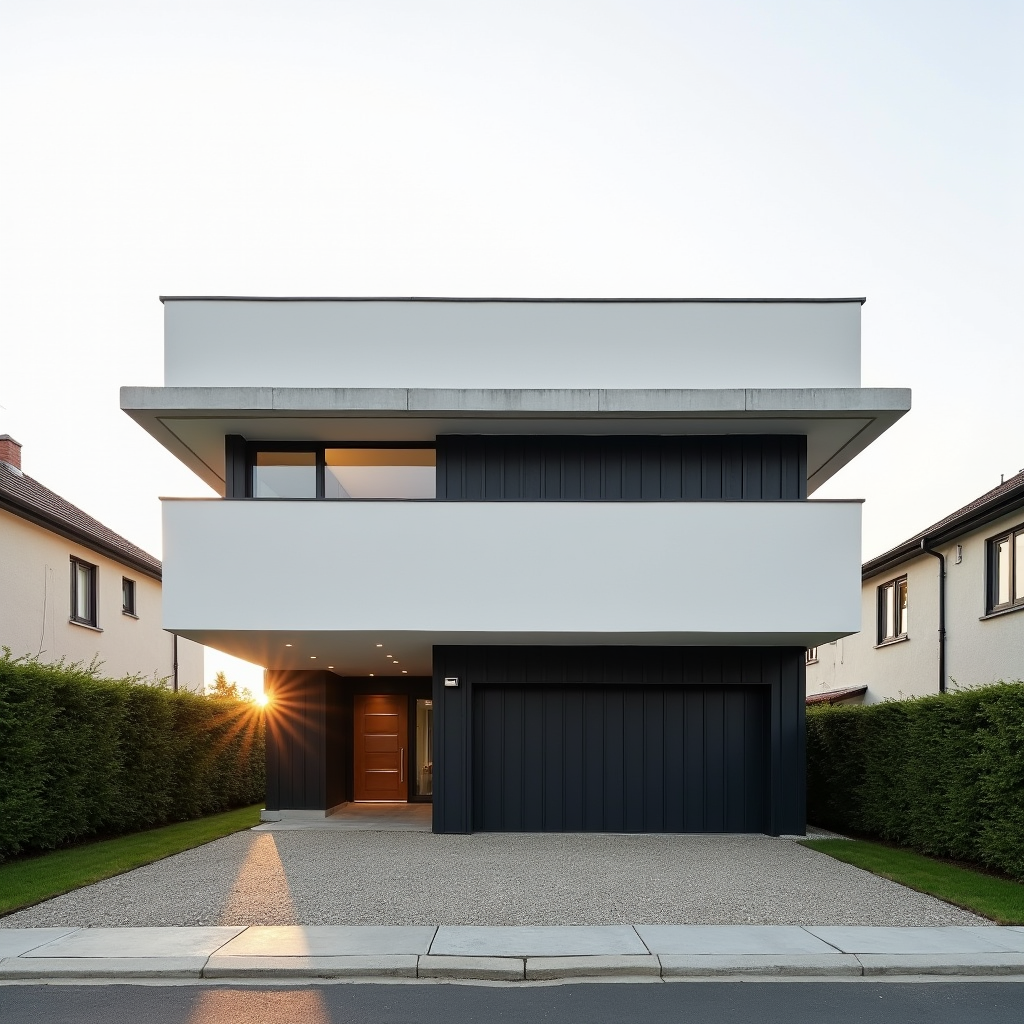
\includegraphics[width=0.12\textwidth]{Images/Results/Architect-A_Fixed-images/2-preliminary_design/Zonder_lora_00069_ (1).png} &
    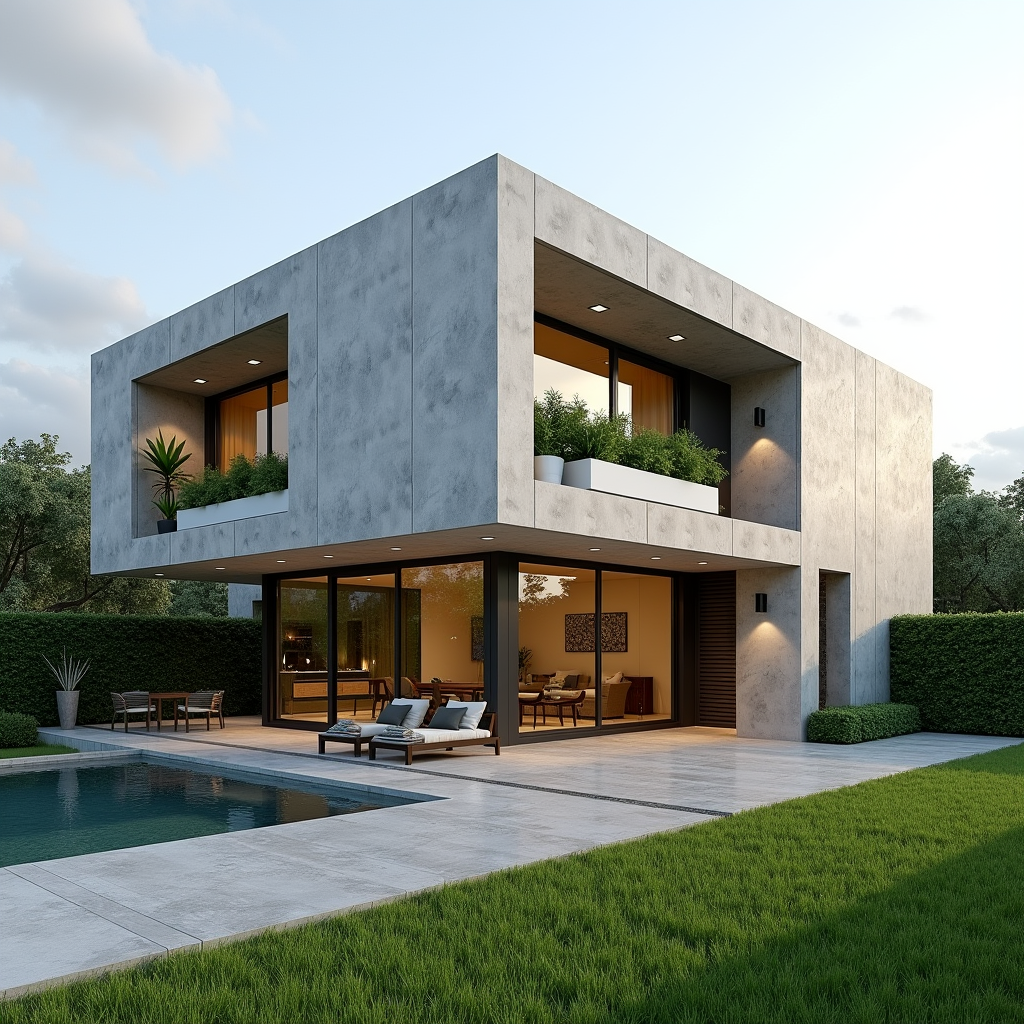
\includegraphics[width=0.12\textwidth]{Images/Results/Architect-A_Fixed-images/2-preliminary_design/Zonder_lora_00080_.png} &
    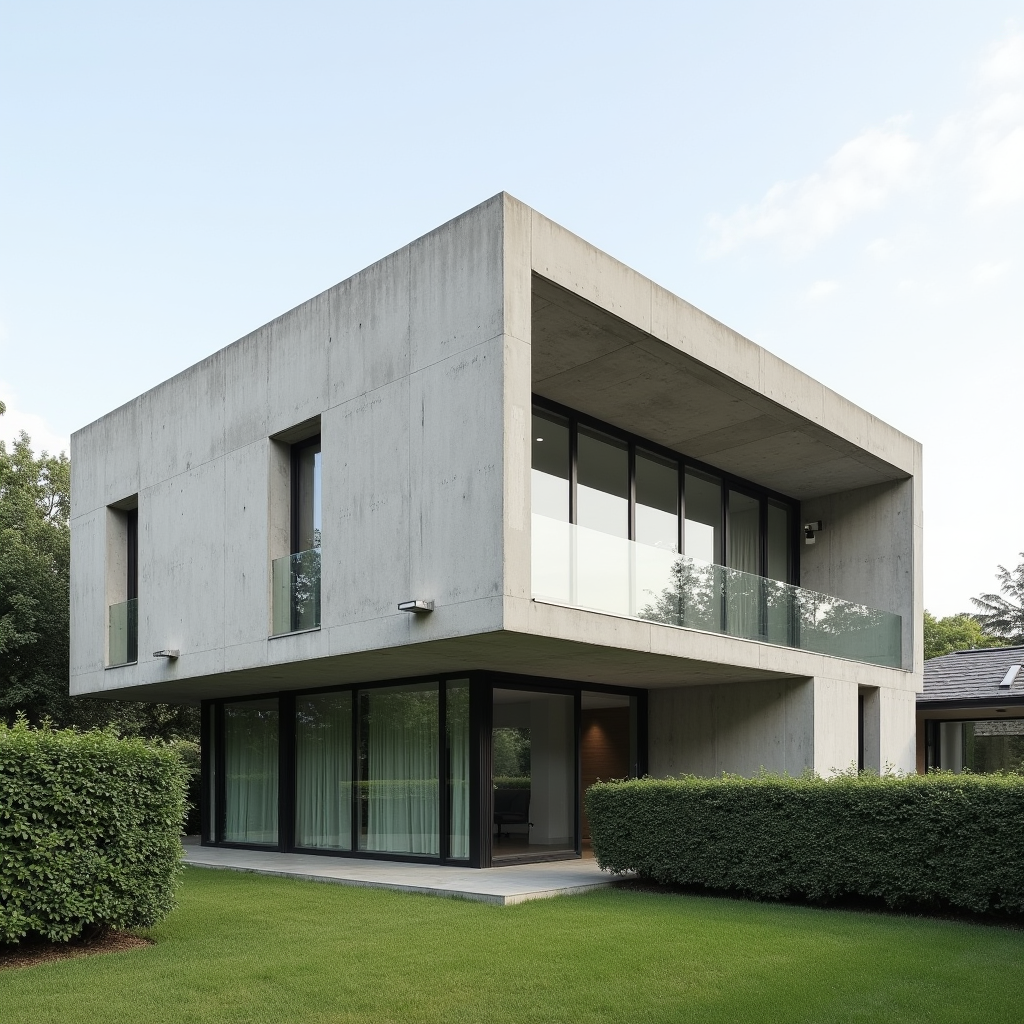
\includegraphics[width=0.12\textwidth]{Images/Results/Architect-A_Fixed-images/2-preliminary_design/Zonder_lora_00089_.png} &
    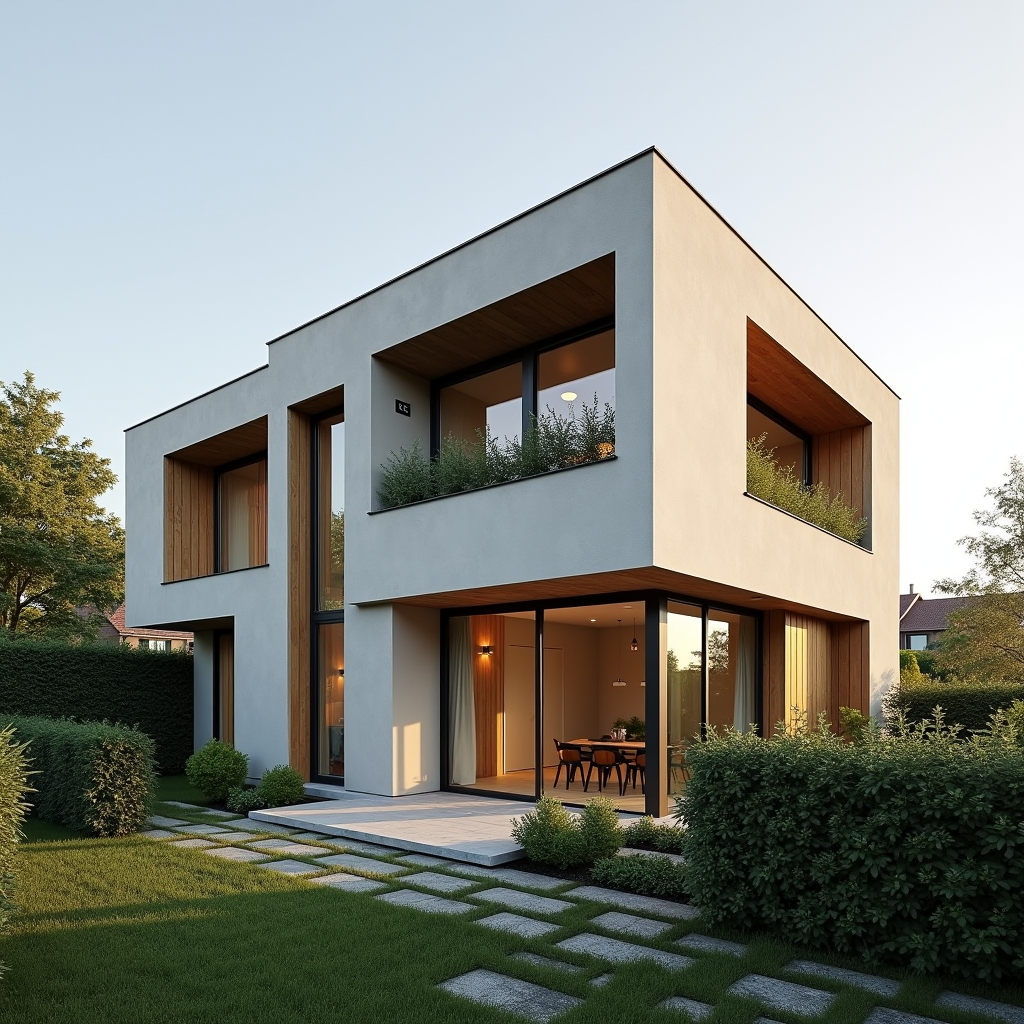
\includegraphics[width=0.12\textwidth]{Images/Results/Architect-A_Fixed-images/2-preliminary_design/Zonder_lora_00091_.png} &
    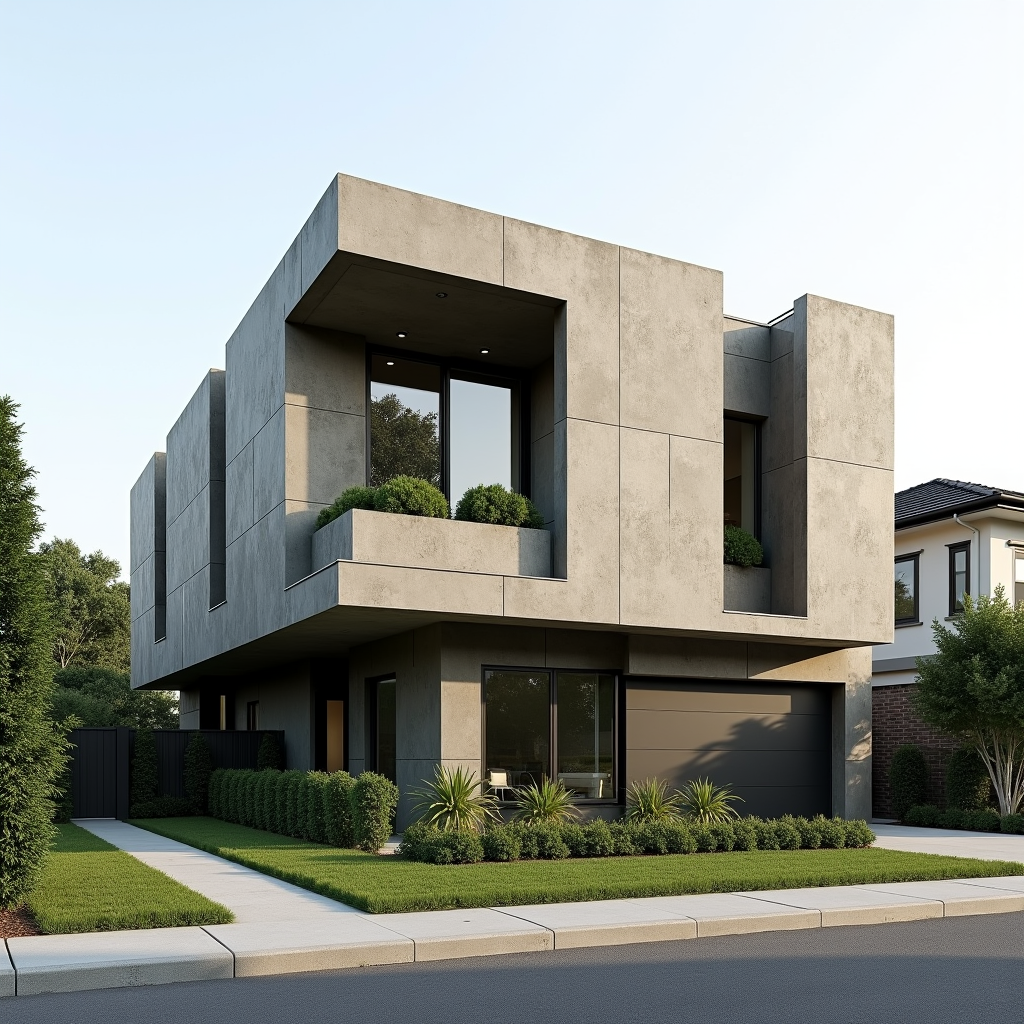
\includegraphics[width=0.12\textwidth]{Images/Results/Architect-A_Fixed-images/2-preliminary_design/Zonder_lora_00095_.png} \\
  \end{tabular}
  }
  \caption{Starting images in the preliminary design phase of architect A.}
  \label{fig:horizontal-lora-comparison}
\end{figure}
\subsubsection{Selected starting image}
Architect A selected the image in figure \ref{fig:A-preliminary-selected}, which was generated with the \textbf{stampbeton} and \textbf{3D-effect} models. 
\begin{figure}[H]
    \centering
    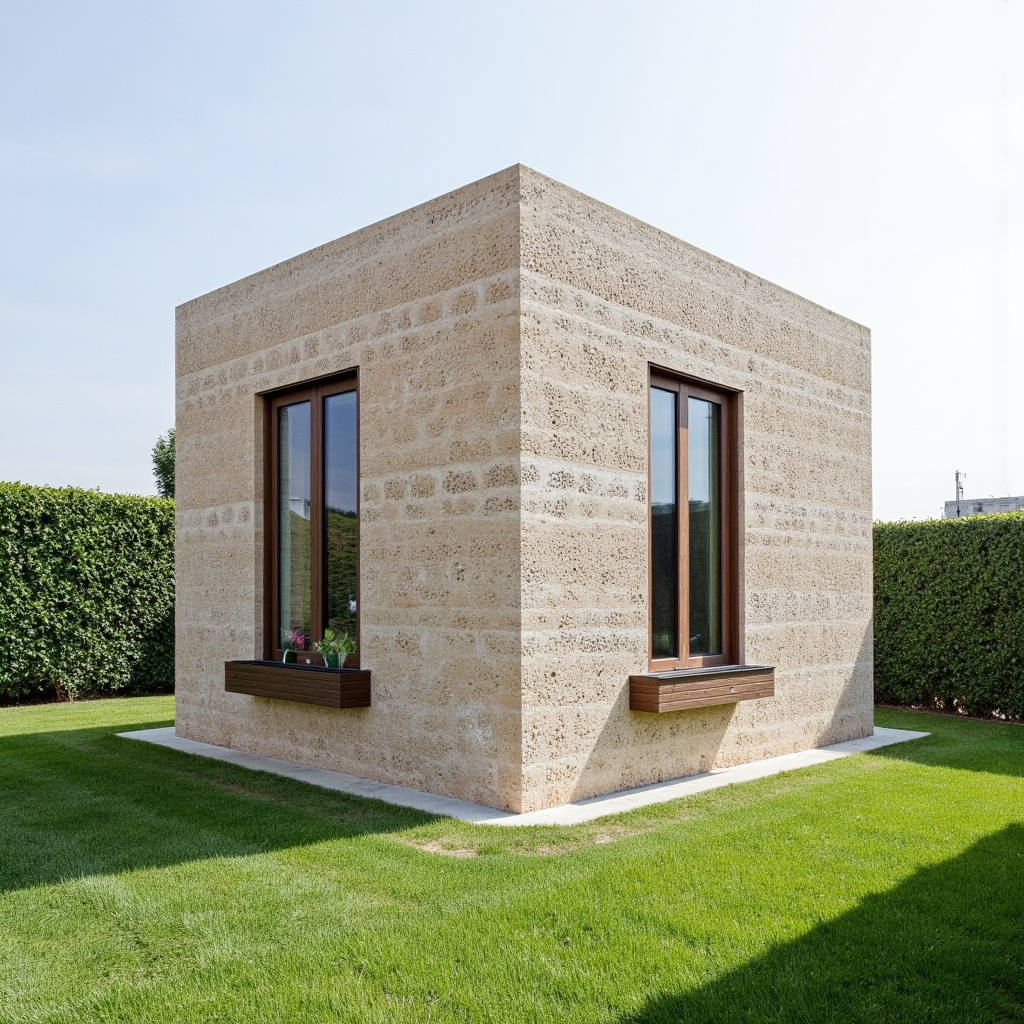
\includegraphics[width=0.3\linewidth]{Images/Results/Architect-A_Fixed-images/2-preliminary_design/Met_lora_00080_.png}
    \caption{Architect A's selected starting image for the preliminary design phase.}
    \label{fig:A-preliminary-selected}
\end{figure}
\subsubsection{Preferred generated images}
Architect A chose two preferred images among the images generated during this design phase. 
\begin{itemize}
    \item Image 1 was created with LoRAs. Architect A chose this image because
    \item Image 2 was created without LoRAs. Architect A chose this image because 
\end{itemize}
\begin{figure}[H]
    \centering
    \begin{tabular}{cc}
         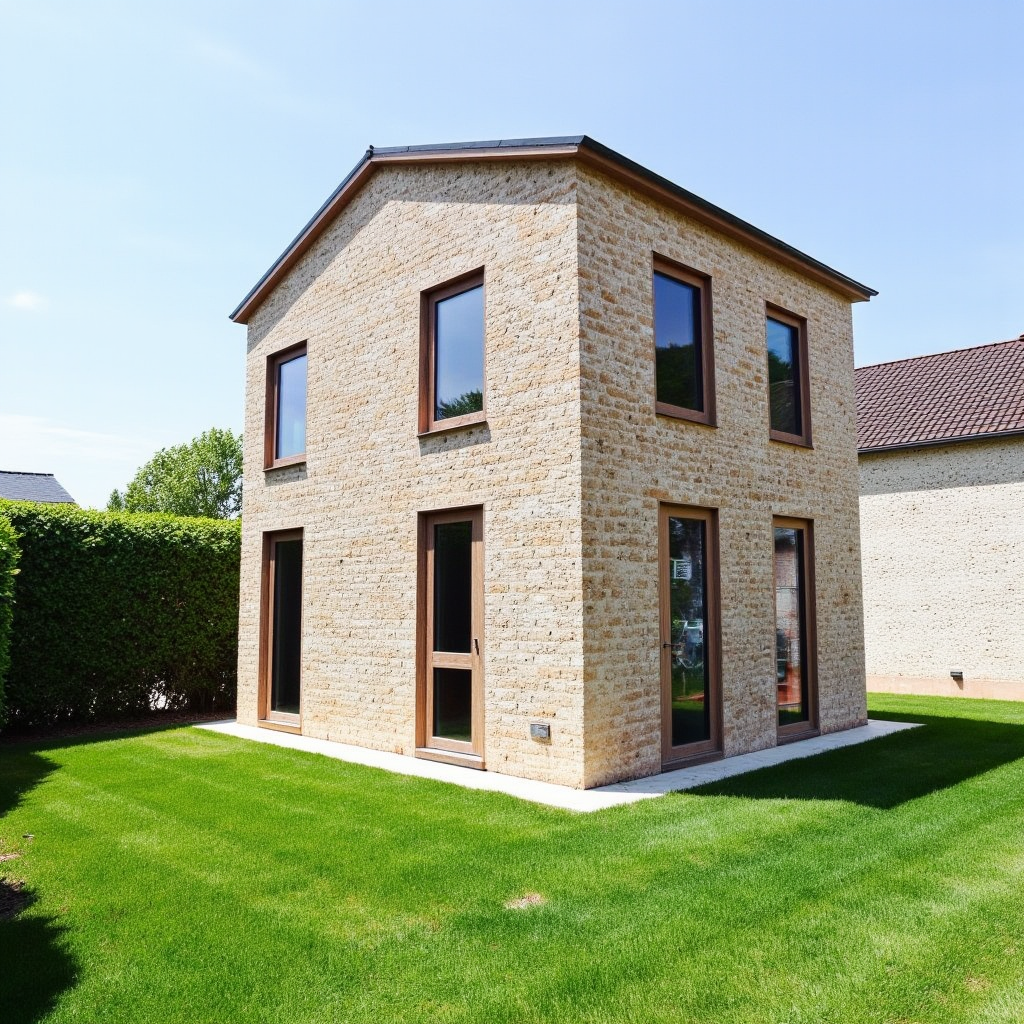
\includegraphics[width=0.3\linewidth]{Images/Results/Architect A/2. Preliminary phase/Met_lora_00004_.png} & 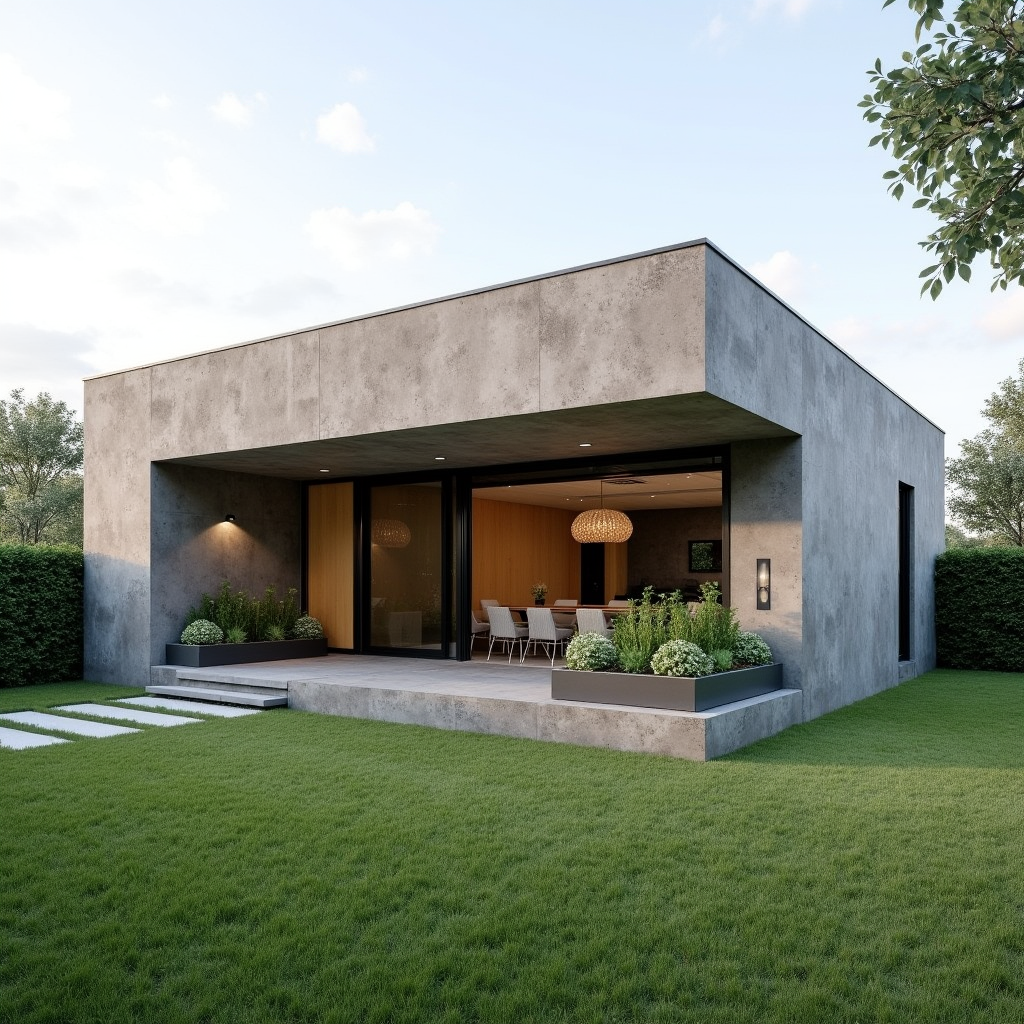
\includegraphics[width=0.3\linewidth]{Images/Results/Architect A/2. Preliminary phase/Zonder_lora_00146_.png}\\
         \textit{(1)} & \textit{(2)}
    \end{tabular}
    \caption{Architect A's favourite images in the preliminary design phase.}
    \label{fig:A-preliminary-preferred}
\end{figure}

\subsection{Presentation phase}
\subsubsection{Starting images}
\begin{figure}[H]
  \centering
  {\footnotesize
  \renewcommand{\arraystretch}{1.1}
  \setlength{\tabcolsep}{4pt}
  \begin{tabular}{c c c c c c c c}
    & \shortstack{\textbf{Stamp-}\\\textbf{beton}} 
    & \shortstack{\textbf{3D-}\\\textbf{effect}} 
    & \textbf{Geleding} 
    & \shortstack{\textbf{Stampbeton}\\ \textbf{\& 3D-effect}} 
    & \shortstack{\textbf{Stampbeton}\\ \textbf{\& Geleding}} 
    & \shortstack{\textbf{3D-effect} \&\\ \textbf{Geleding}} 
    & \shortstack{\textbf{Stampbeton,}\\\textbf{3D-effect \&}\\\textbf{Geleding}} \\

    \shortstack{\textbf{With}\\\textbf{LoRA}} & 
    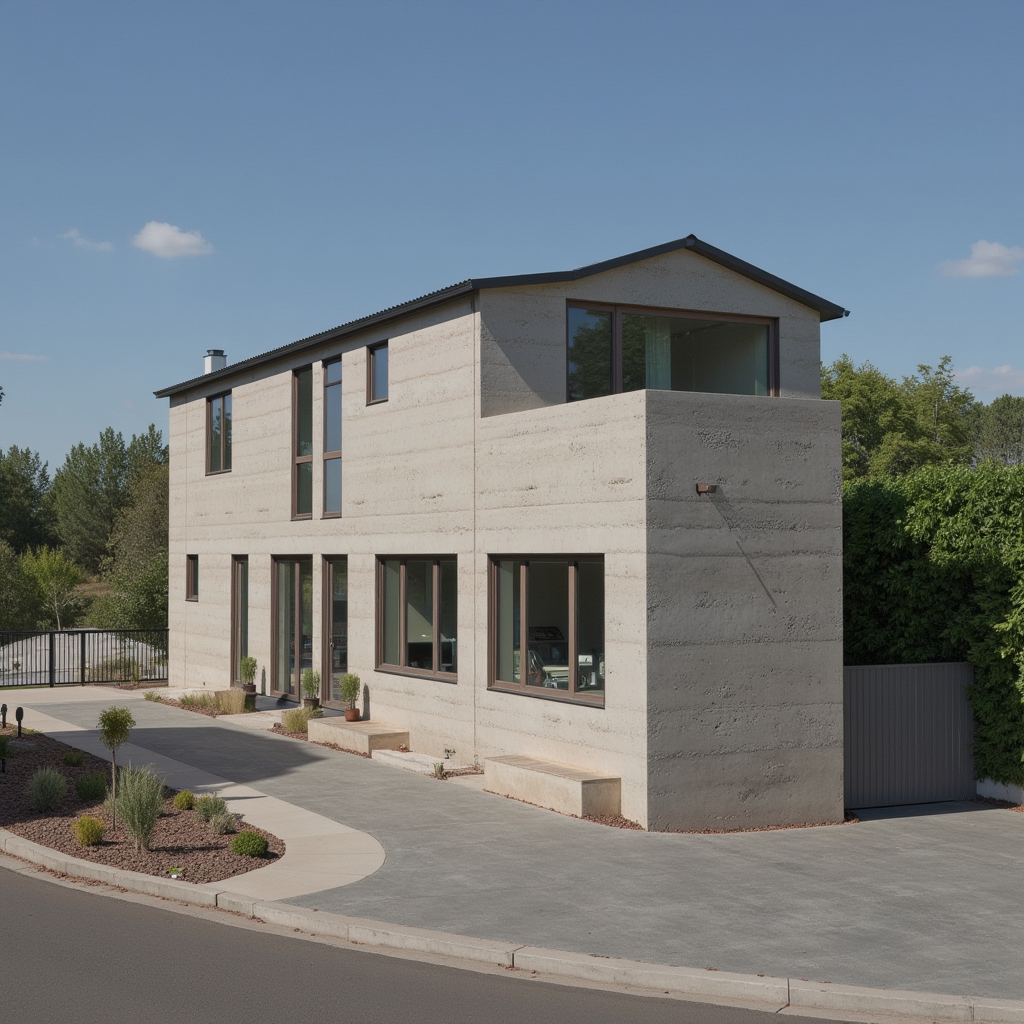
\includegraphics[width=0.12\textwidth]{Images/Results/Architect-A_Fixed-images/3-presentation/Met_lora_00097_.png} & 
    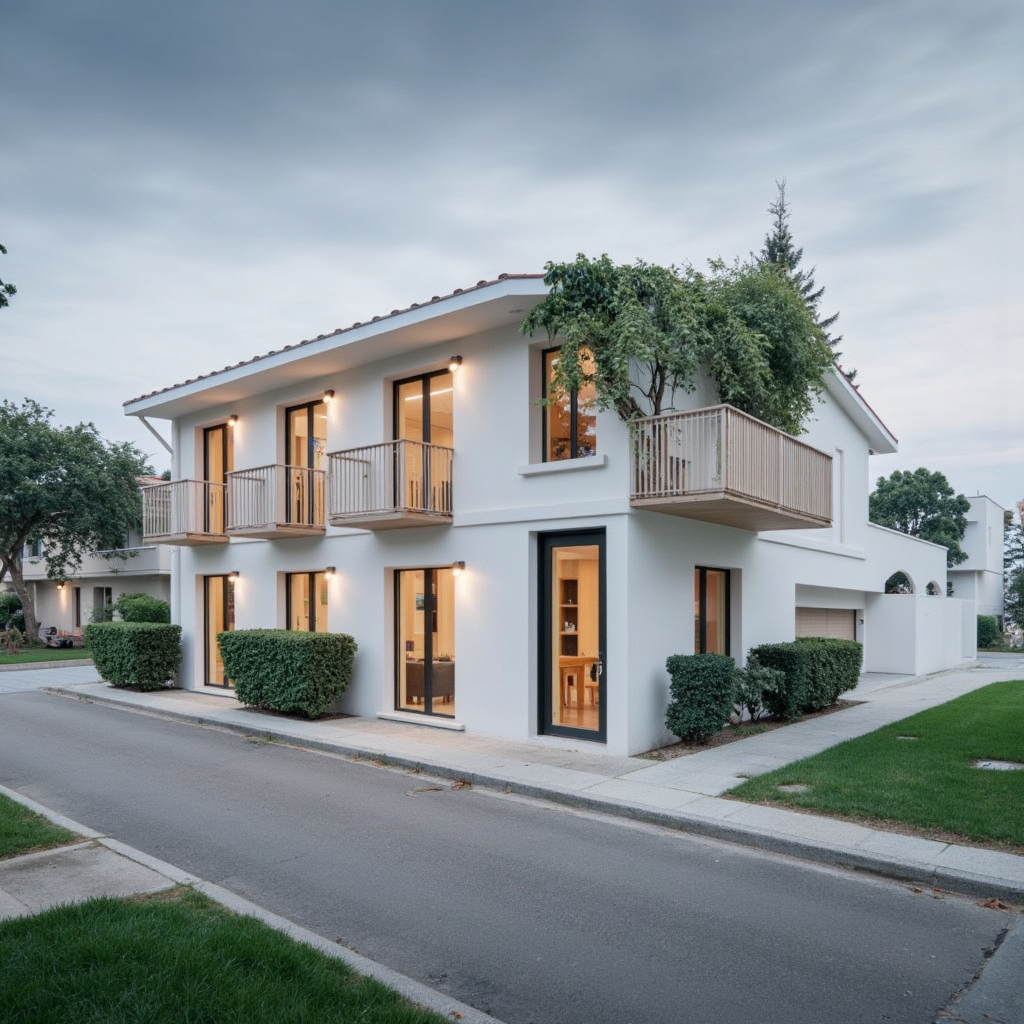
\includegraphics[width=0.12\textwidth]{Images/Results/Architect-A_Fixed-images/3-presentation/Met_lora_00100_.png} &
    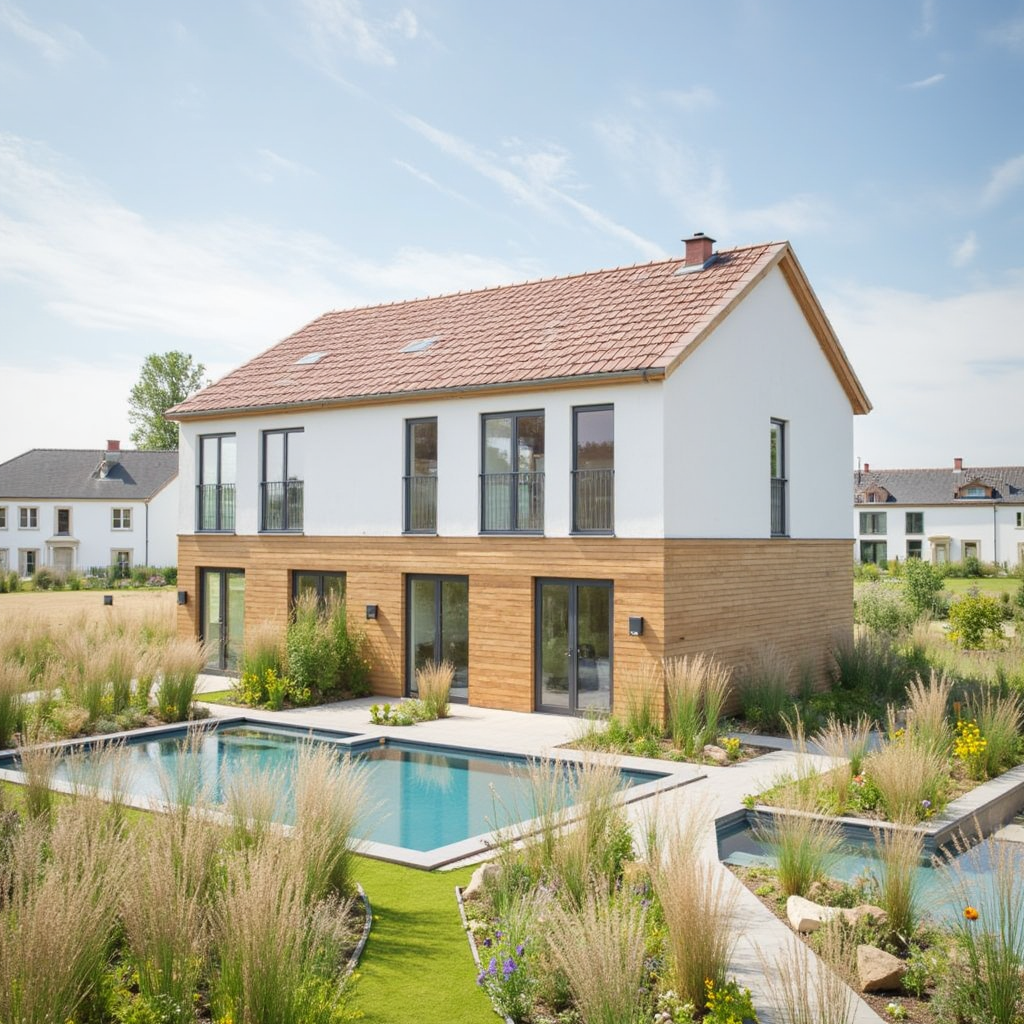
\includegraphics[width=0.12\textwidth]{Images/Results/Architect-A_Fixed-images/3-presentation/Met_lora_00106_.png} &
    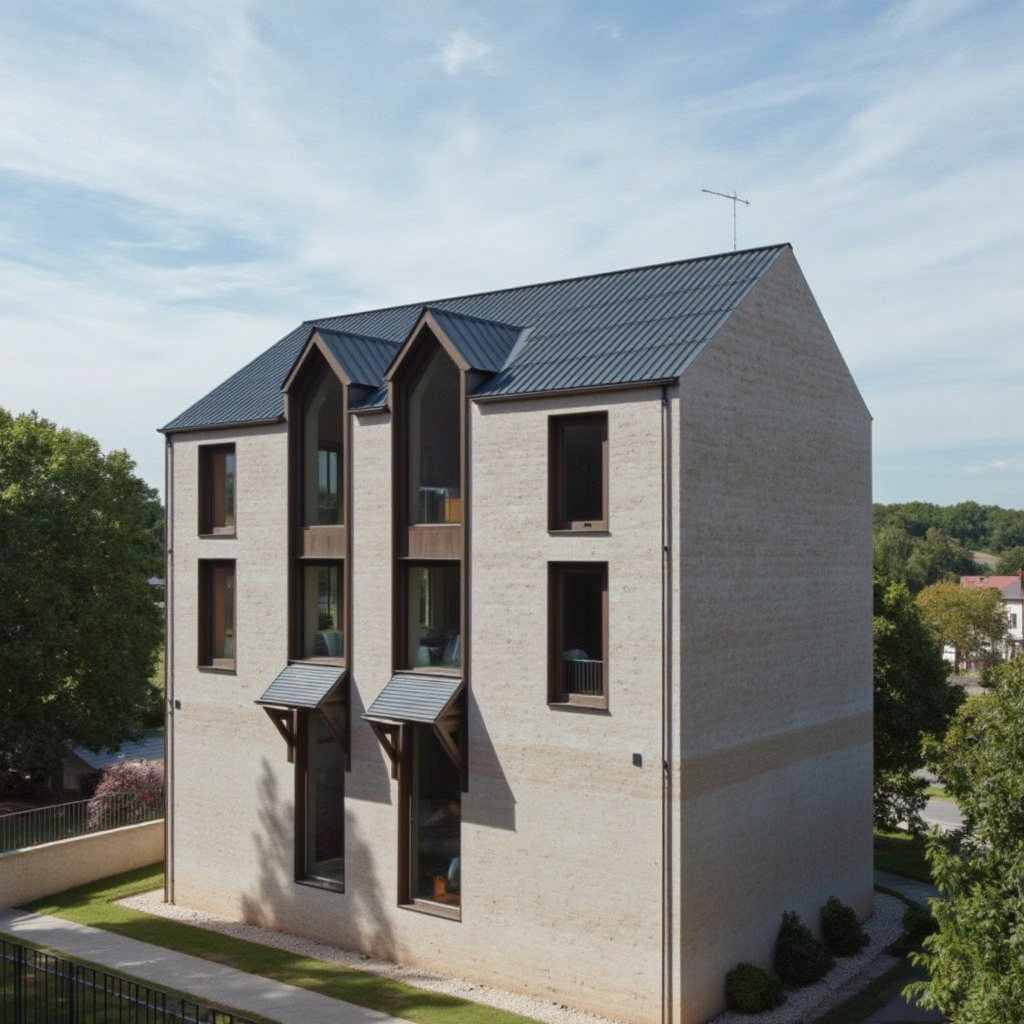
\includegraphics[width=0.12\textwidth]{Images/Results/Architect-A_Fixed-images/3-presentation/Met_lora_00111_.png} &
    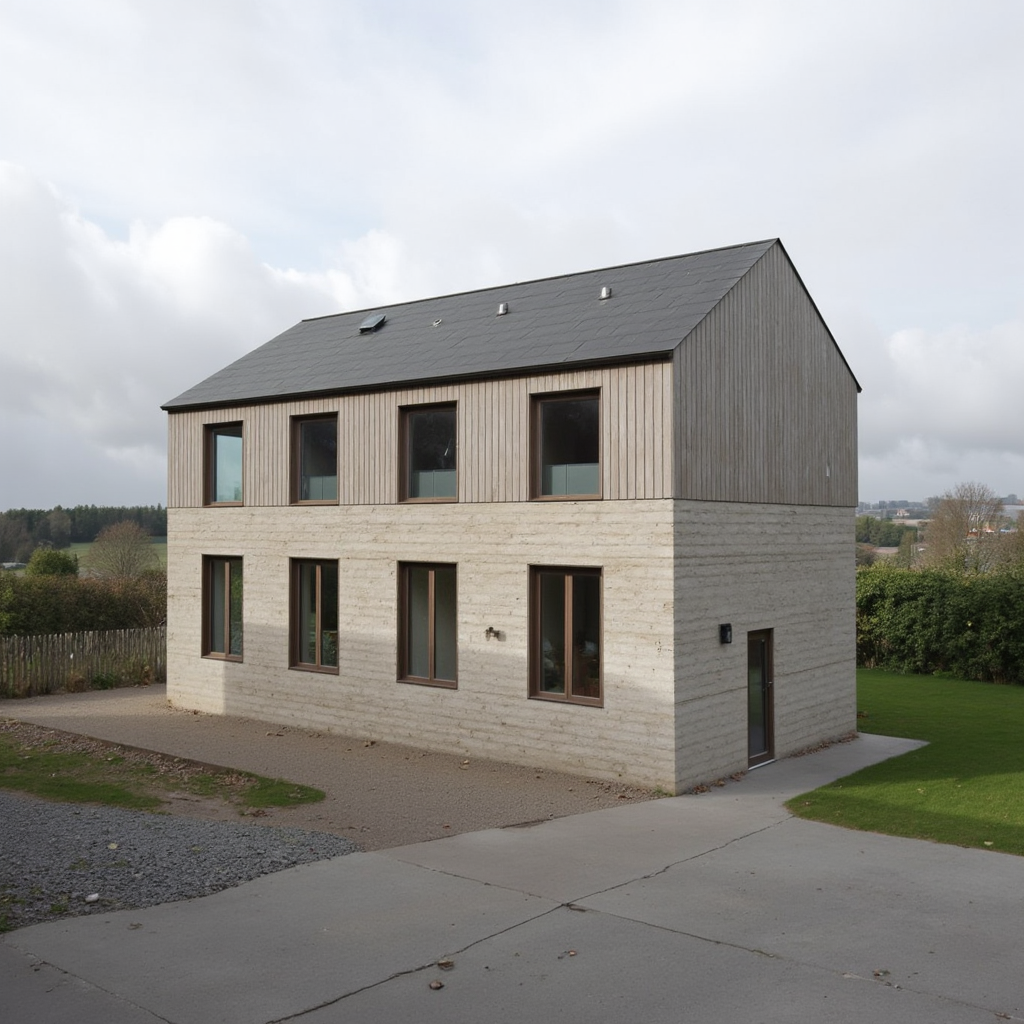
\includegraphics[width=0.12\textwidth]{Images/Results/Architect-A_Fixed-images/3-presentation/Met_lora_00115_.png} &
    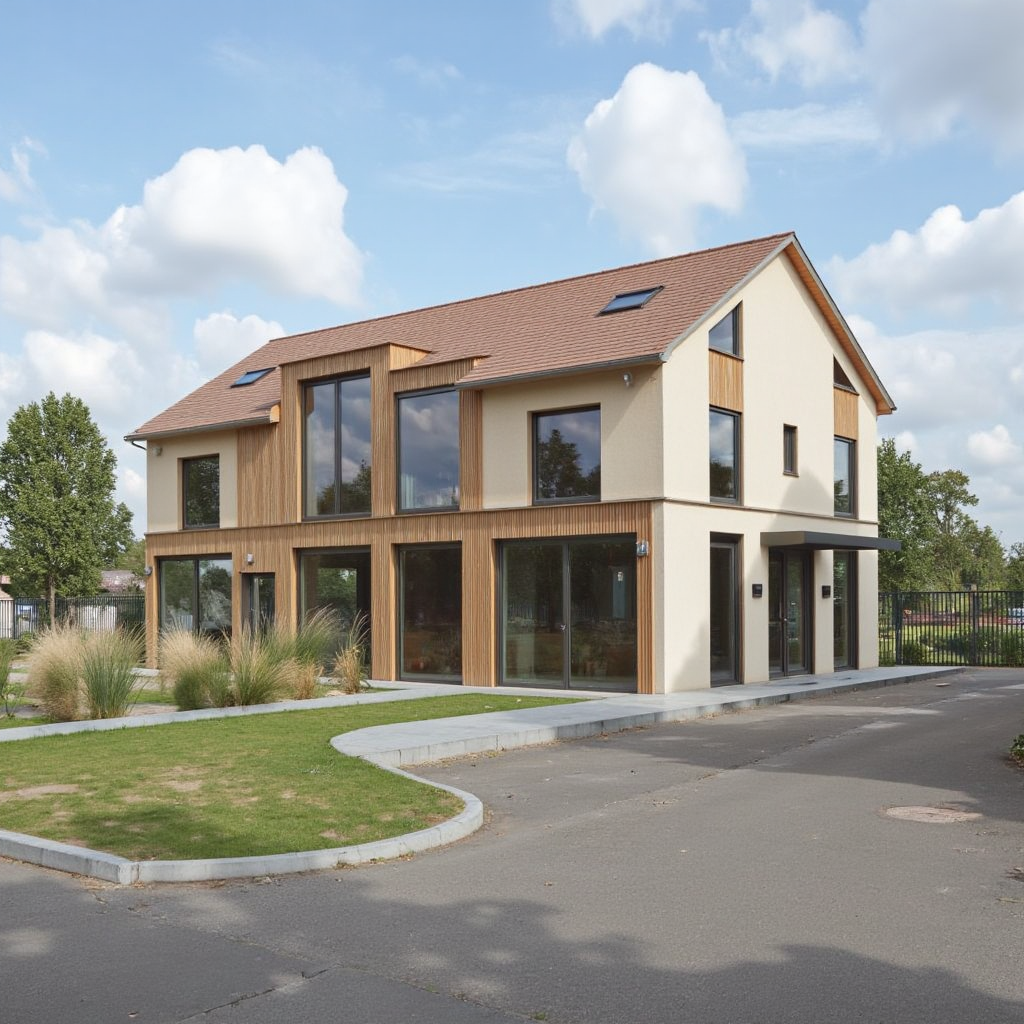
\includegraphics[width=0.12\textwidth]{Images/Results/Architect-A_Fixed-images/3-presentation/Met_lora_00117_.png} &
    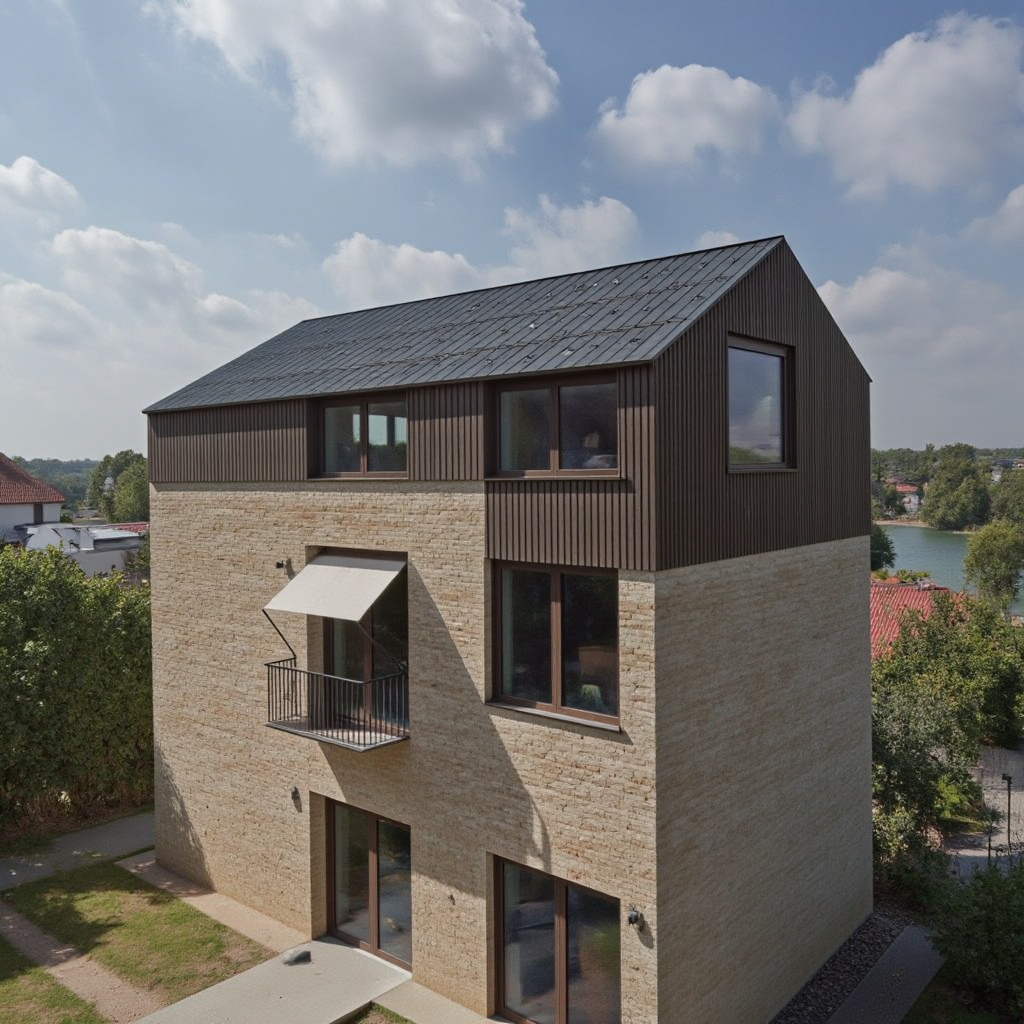
\includegraphics[width=0.12\textwidth]{Images/Results/Architect-A_Fixed-images/3-presentation/Met_lora_00121_.png} \\

    \shortstack{\textbf{Without}\\\textbf{LoRA}} &
    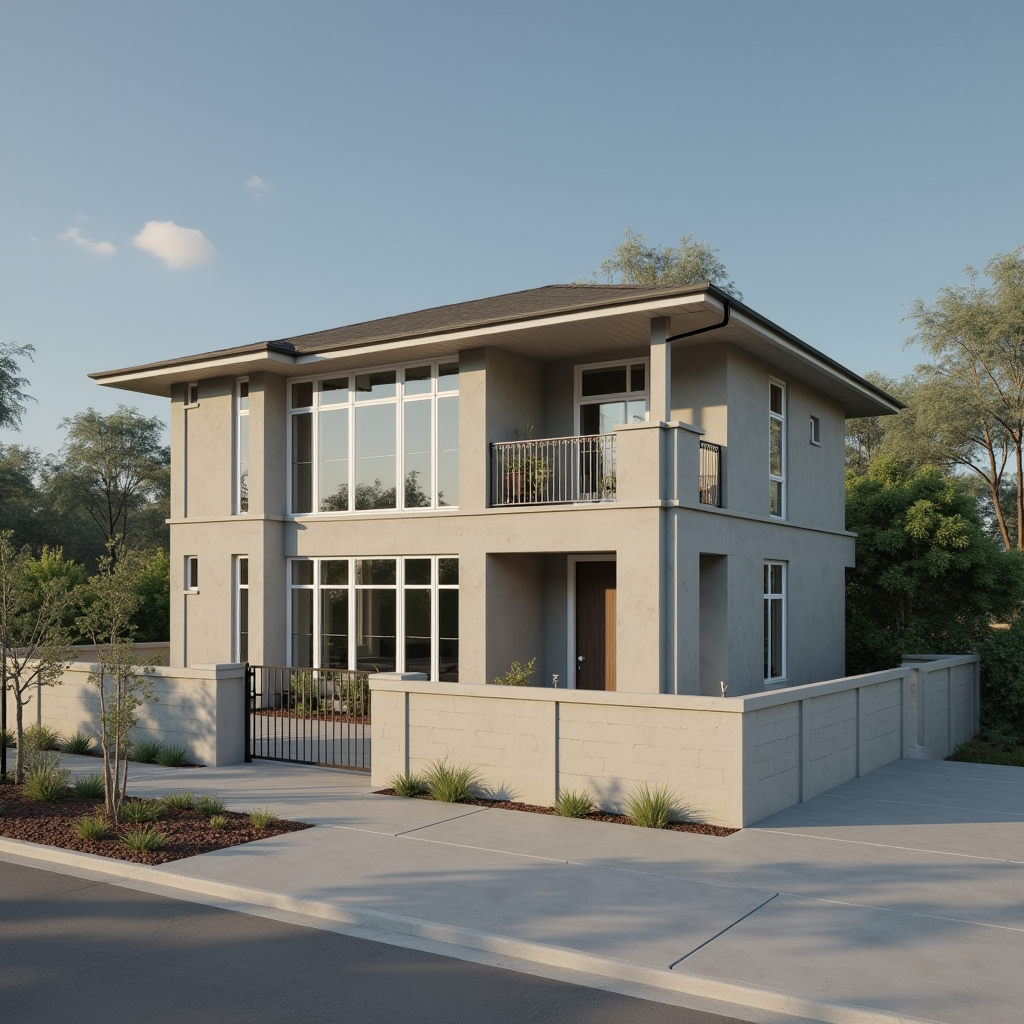
\includegraphics[width=0.12\textwidth]{Images/Results/Architect-A_Fixed-images/3-presentation/Zonder_lora_00097_.png} &
    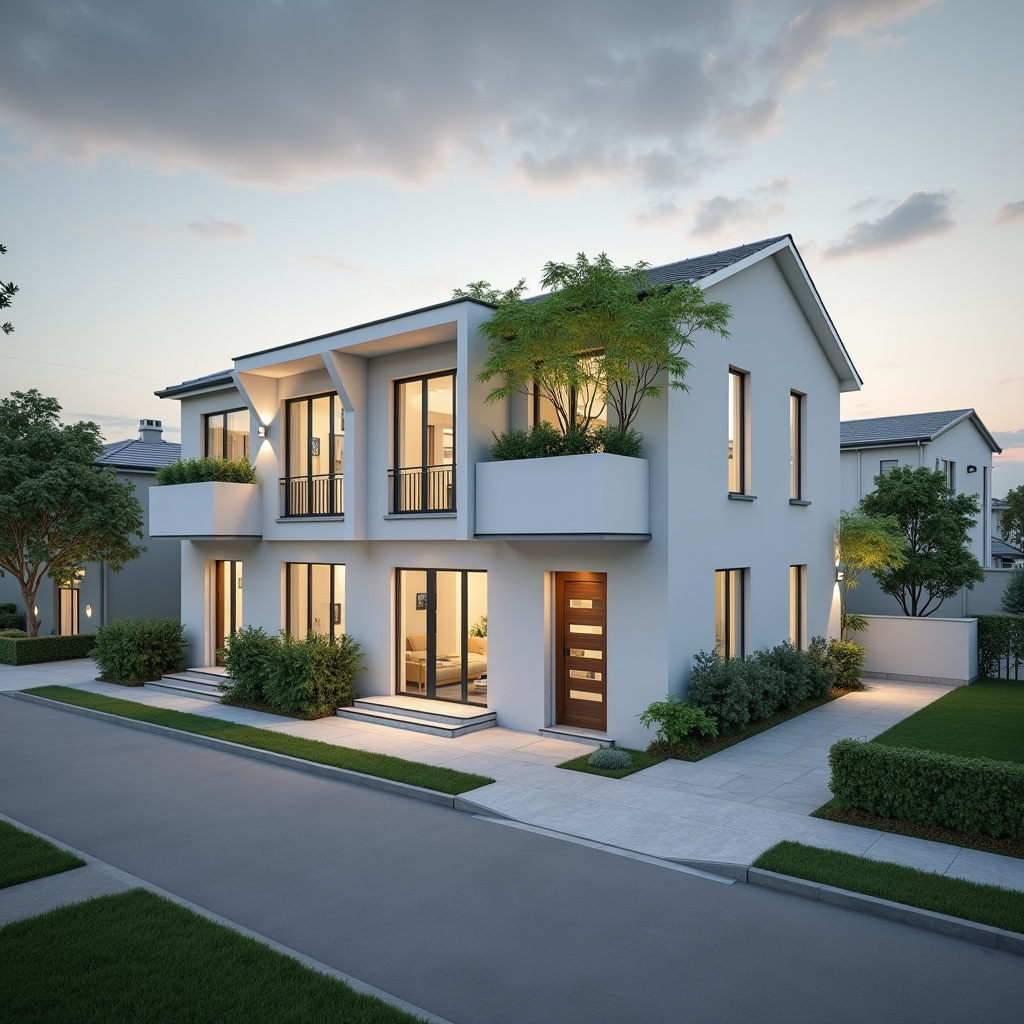
\includegraphics[width=0.12\textwidth]{Images/Results/Architect-A_Fixed-images/3-presentation/Zonder_lora_00100_.png} &
    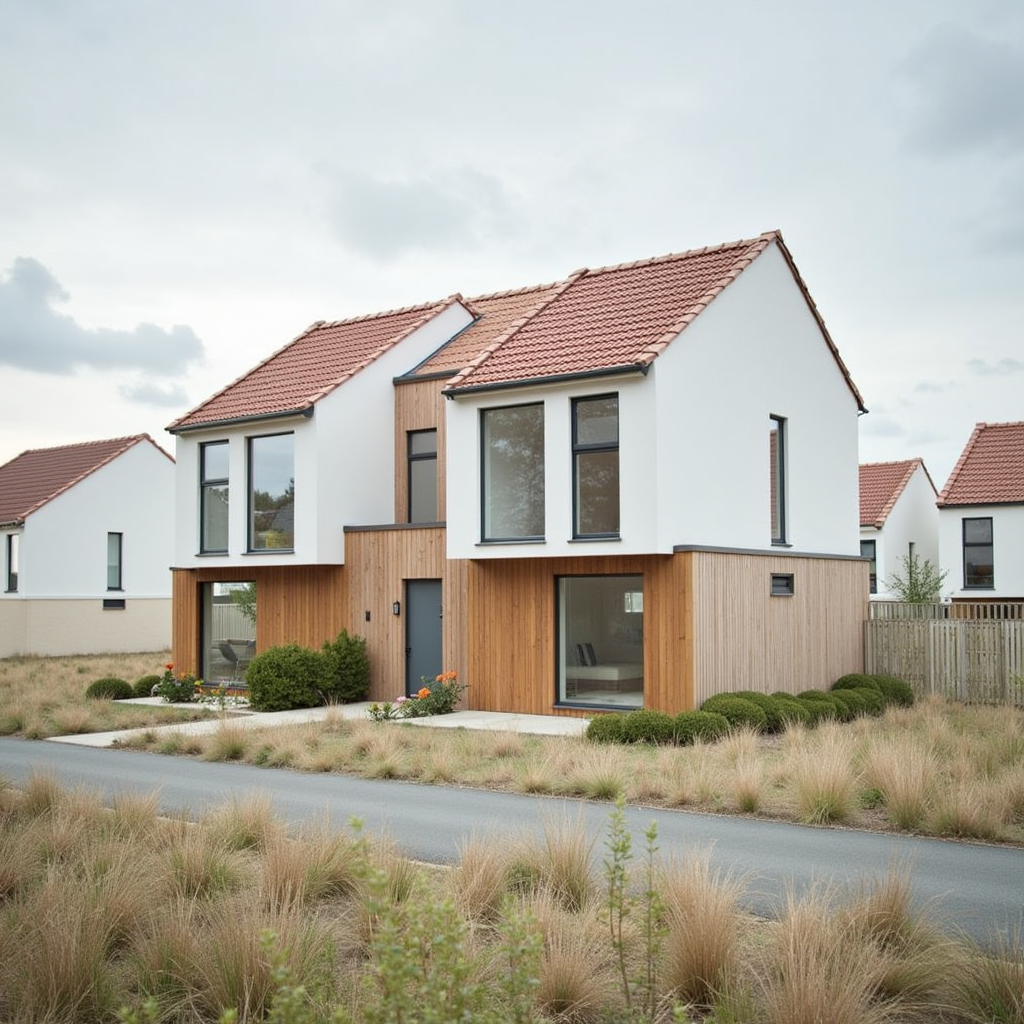
\includegraphics[width=0.12\textwidth]{Images/Results/Architect-A_Fixed-images/3-presentation/Zonder_lora_00106_.png} &
    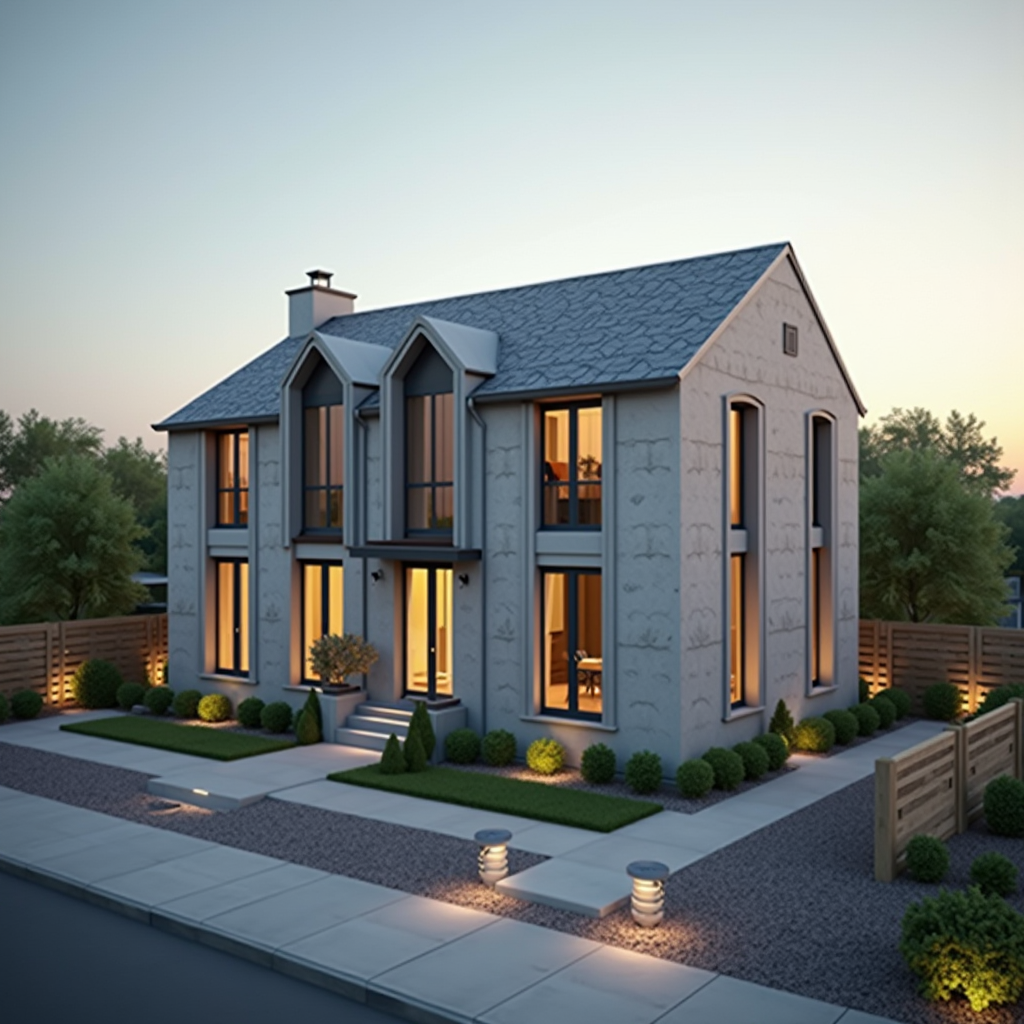
\includegraphics[width=0.12\textwidth]{Images/Results/Architect-A_Fixed-images/3-presentation/Zonder_lora_00111_.png} &
    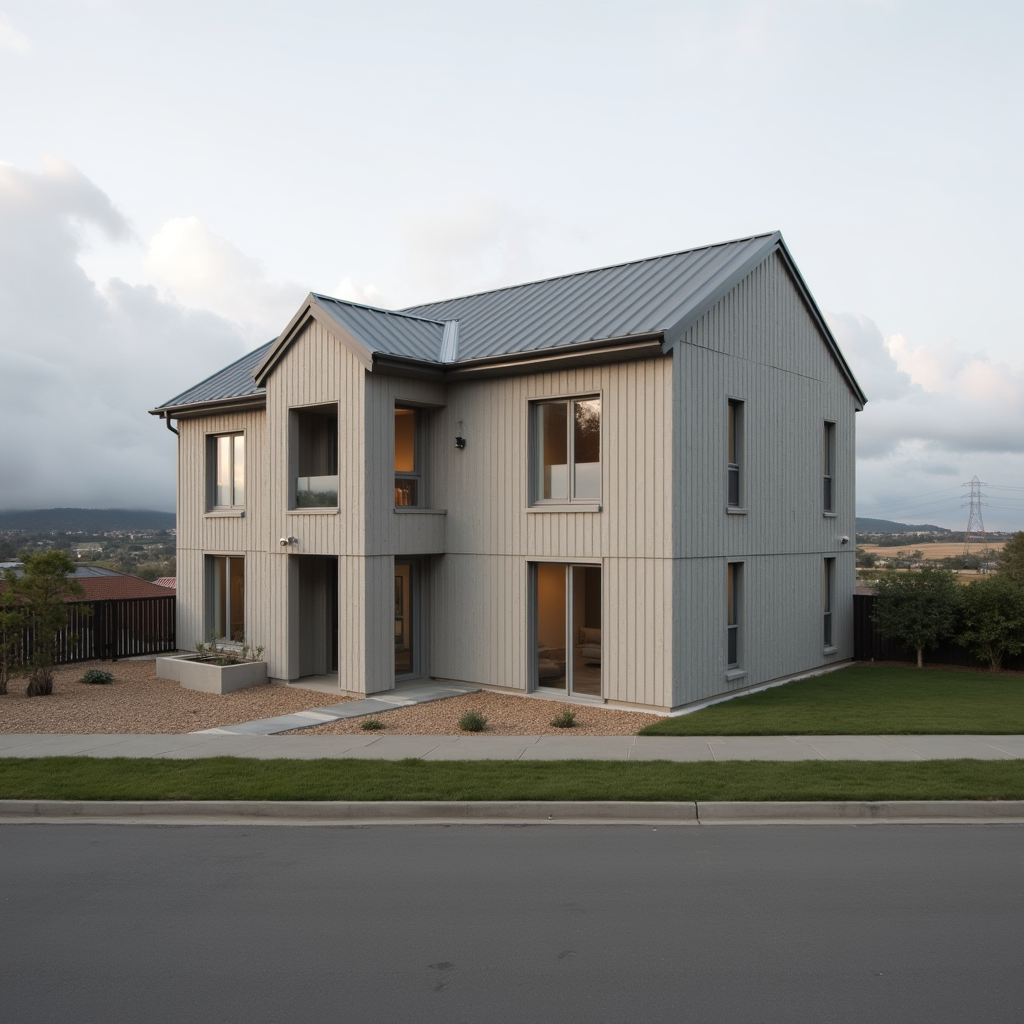
\includegraphics[width=0.12\textwidth]{Images/Results/Architect-A_Fixed-images/3-presentation/Zonder_lora_00115_.png} &
    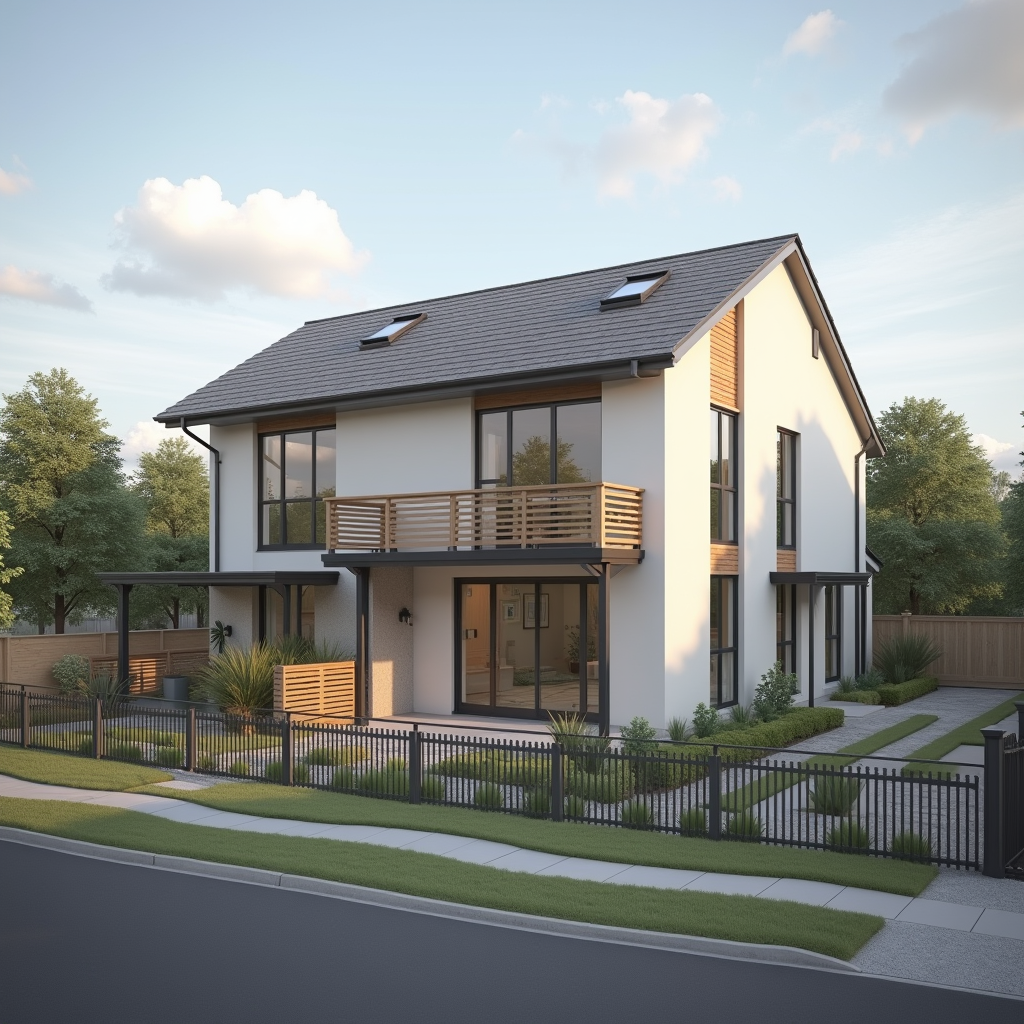
\includegraphics[width=0.12\textwidth]{Images/Results/Architect-A_Fixed-images/3-presentation/Zonder_lora_00117_.png} &
    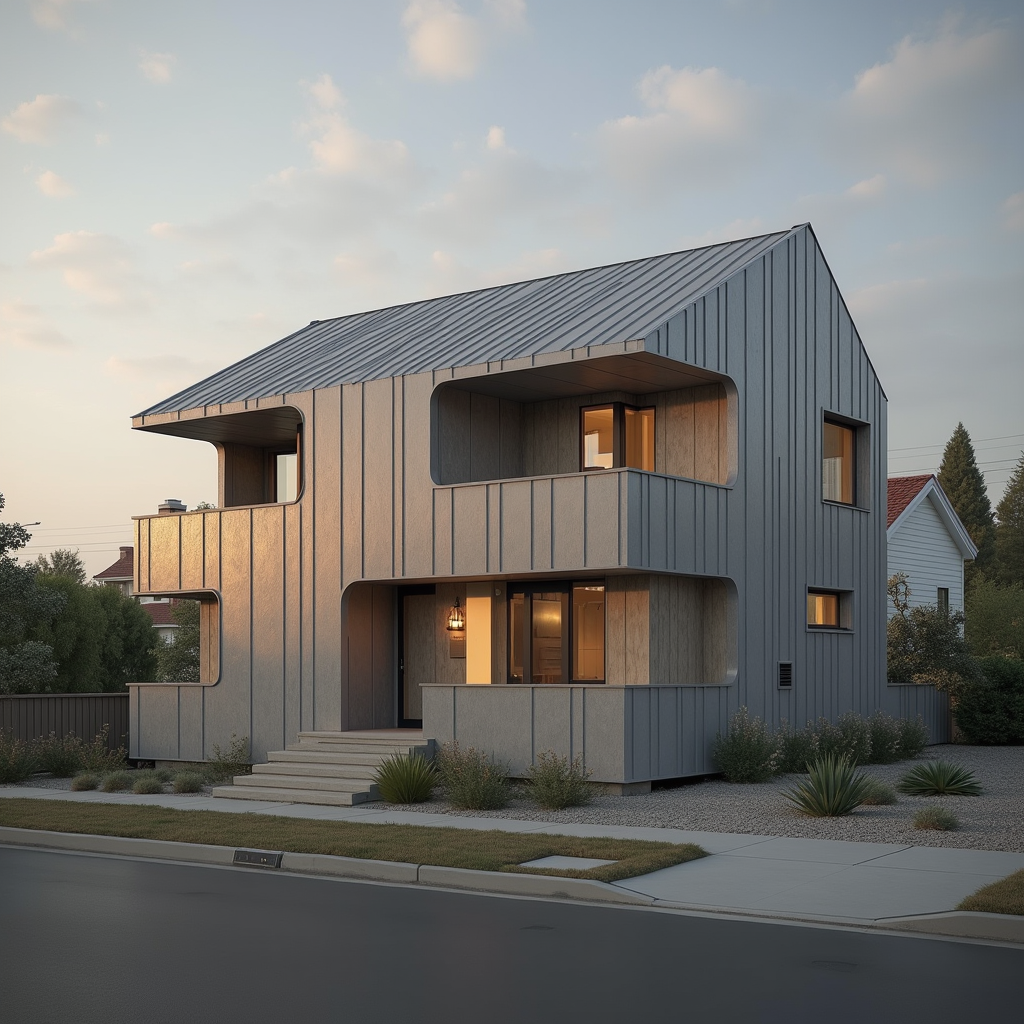
\includegraphics[width=0.12\textwidth]{Images/Results/Architect-A_Fixed-images/3-presentation/Zonder_lora_00121_.png} \\
  \end{tabular}
  }
  \caption{Starting images in the presentation phase of architect A.}
  \label{fig:horizontal-lora-comparison}
\end{figure}

\subsubsection{Selected starting image}
Architect A selected the image in figure \ref{fig:A-presentation-selected} , which was generated with the stampbeton LoRA. His reasons were the beautiful stamped concrete, and the interaction of the building with the environment. He could 'imagine an interesting location plan'. Additionally, the unusual shape of the roof 'suggests something below it' and 'allows for fun spaces inside'.
\begin{figure}[H]
    \centering
    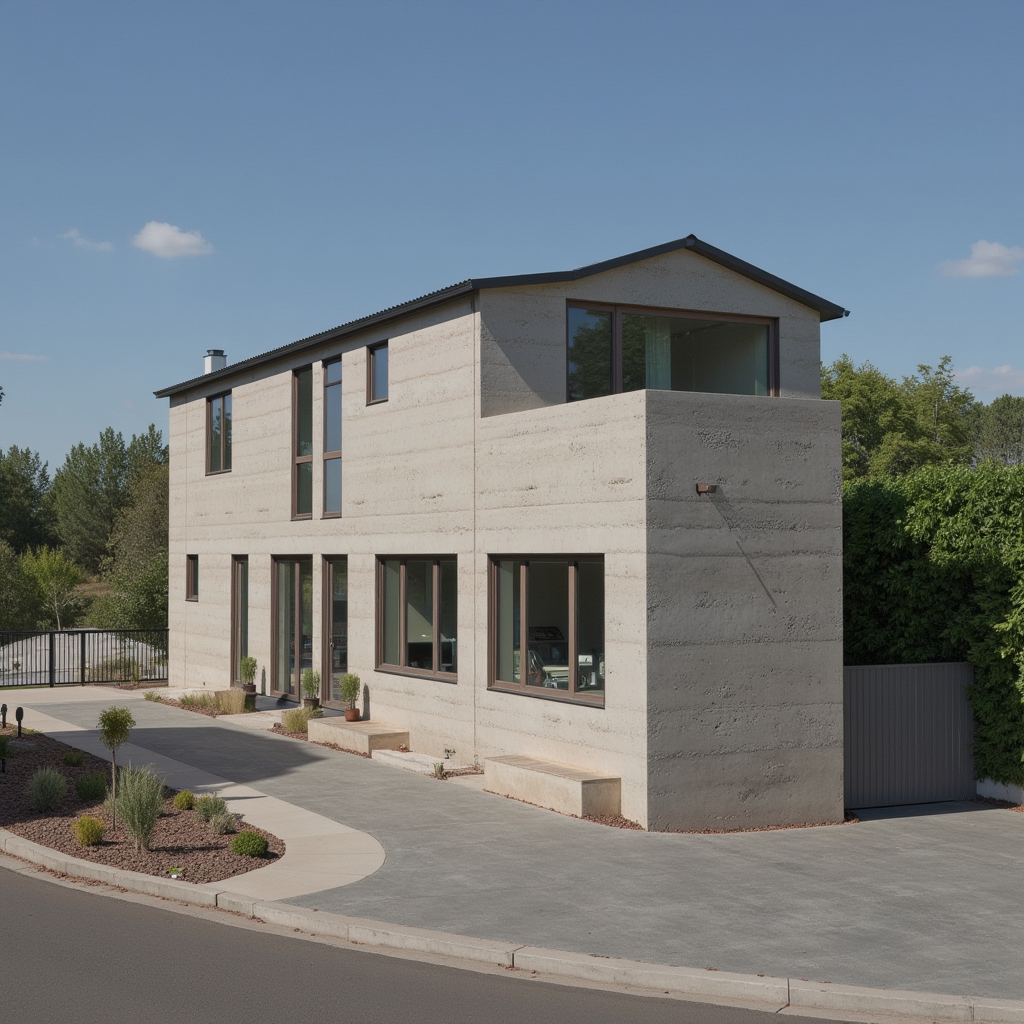
\includegraphics[width=0.3\linewidth]{Images/Results/Architect-A_Fixed-images/3-presentation/Met_lora_00097_.png}
    \caption{Architect A's selected starting image for the presentation phase.}
    \label{fig:A-presentation-selected}
\end{figure}

\subsubsection{Preferred generated images}
Architect A chose two preferred images among the images generated during this design phase. Both images were created with LoRA.
\begin{figure}[H]
    \centering
    \begin{tabular}{cc}
        \includegraphics[width=0.3\textwidth]{Images/Results/Architect A/3. Presentation phase/Met_lora_00002_.png} & \includegraphics[width=0.3\textwidth]{Images/Results/Architect A/3. Presentation phase/Met_lora_00006_.png}\\ 
        (1) & (2)\\
    \end{tabular}
    \caption{Architect A's preferred images in the presentation phase.}
    \label{fig:A-presentation-preferred}
\end{figure}
\subsection{Free phase}

\section{Architect B}
\subsection{Sketch design phase}
\subsubsection{Starting images}
\begin{figure}[H]
  \centering
  {\footnotesize
  \renewcommand{\arraystretch}{1.1}
  \setlength{\tabcolsep}{4pt}
  \begin{tabular}{c c c c c c c c}
    & \textbf{Ghoek} & \textbf{Modulariteit} & \shortstack{\textbf{Plint-}\\\textbf{werking}}
    & \shortstack{\textbf{Ghoek \&}\\ \textbf{modulari-}\\\textbf{teit}} 
    & \shortstack{\textbf{Ghoek \&}\\ \textbf{Plintwerking}} 
    & \shortstack{\textbf{Modulariteit} \\ \textbf{ \& Plint-}\\\textbf{werking}} 
    & \shortstack{\textbf{Ghoek,}\\\textbf{Modulari-}\\\textbf{teit \&}\\\textbf{PLintwerking}} \\

    \shortstack{\textbf{With}\\\textbf{LoRA}} & 
    \includegraphics[width=0.12\textwidth]{Images/Results/Architect-B_Fixed-images/1-sketch_design/Met_lora_00004_.png} & 
    \includegraphics[width=0.12\textwidth]{Images/Results/Architect-B_Fixed-images/1-sketch_design/Met_lora_00007_.png} &
    \includegraphics[width=0.12\textwidth]{Images/Results/Architect-B_Fixed-images/1-sketch_design/Met_lora_00010_.png} &
    \includegraphics[width=0.12\textwidth]{Images/Results/Architect-B_Fixed-images/1-sketch_design/Met_lora_00017_.png} &
    \includegraphics[width=0.12\textwidth]{Images/Results/Architect-B_Fixed-images/1-sketch_design/Met_lora_00021_.png} &
    \includegraphics[width=0.12\textwidth]{Images/Results/Architect-B_Fixed-images/1-sketch_design/Met_lora_00024_.png} &
    \includegraphics[width=0.12\textwidth]{Images/Results/Architect-B_Fixed-images/1-sketch_design/Met_lora_00026_.png} \\

    \shortstack{\textbf{Without}\\\textbf{LoRA}} &
    \includegraphics[width=0.12\textwidth]{Images/Results/Architect-B_Fixed-images/1-sketch_design/Zonder_lora_00004_.png} &
    \includegraphics[width=0.12\textwidth]{Images/Results/Architect-B_Fixed-images/1-sketch_design/Zonder_lora_00007_.png} &
    \includegraphics[width=0.12\textwidth]{Images/Results/Architect-B_Fixed-images/1-sketch_design/Zonder_lora_00010_.png} &
    \includegraphics[width=0.12\textwidth]{Images/Results/Architect-B_Fixed-images/1-sketch_design/Zonder_lora_00017_.png} &
    \includegraphics[width=0.12\textwidth]{Images/Results/Architect-B_Fixed-images/1-sketch_design/Zonder_lora_00021_.png} &
    \includegraphics[width=0.12\textwidth]{Images/Results/Architect-B_Fixed-images/1-sketch_design/Zonder_lora_00024_.png} &
    \includegraphics[width=0.12\textwidth]{Images/Results/Architect-B_Fixed-images/1-sketch_design/Zonder_lora_00026_.png} \\
  \end{tabular}
  }
  \caption{Starting images in the sketch design phase of architect B.}
  \label{fig:horizontal-lora-comparison}
\end{figure}

\subsubsection{Selected starting image}
Architect B at first selected the image in figure \ref{fig:B-sketch-selected-a}, which was generated without any LoRAs. When told which images were trained and which were not, the architect changed his choice to the image in figure \ref{fig:B-sketch-selected-b}, which was generated with all LoRAs; Ghoek, Modulariteit and Plintwerking.
\begin{figure}[H]
    \centering
    \begin{subfigure}[b]{0.3\textwidth}
        \centering
        \includegraphics[width=\textwidth]{Images/Results/Architect-B_Fixed-images/1-sketch_design/Zonder_lora_00007_.png}
        \caption{}
        \label{fig:B-sketch-selected-a}
    \end{subfigure}
    \begin{subfigure}[b]{0.3\textwidth}
        \centering
        \includegraphics[width=\textwidth]{Images/Results/Architect-B_Fixed-images/1-sketch_design/Met_lora_00026_.png}
        \caption{}
        \label{fig:B-sketch-selected-b}
    \end{subfigure}
    \caption{Architect B's initial and final selected starting image for the sketch design phase.}
    \label{fig:B-sketch-selected}
\end{figure}
\subsubsection{Preferred generated images}
Architect B chose two preferred images among the images generated during this design phase. The image in figure \ref{B-sketch-preferred-a} was created with LoRA, and image \ref{B-sketch-preferred-b} was created without any LoRAs.
\begin{figure}[H]
    \centering
    \begin{subfigure}[b]{0.3\textwidth}
        \centering
        \includegraphics[width=\textwidth]{Images/Results/Architect B/1. Sketch phase/Met_lora_00002_.png}
        \caption{}
        \label{B-sketch-preferred-a}
    \end{subfigure}
    \begin{subfigure}[b]{0.3\textwidth}
        \centering
        \includegraphics[width=\textwidth]{Images/Results/Architect B/1. Sketch phase/Zonder_lora_00002_.png}
        \caption{}
        \label{B-sketch-preferred-b}
    \end{subfigure}
    \caption{Architect B's preferred images in the sketch design phase.}
    \label{fig:B-sketch-preferred}
\end{figure}
\subsection{Preliminary design phase}
\subsubsection{Starting images}
\begin{figure}[H]
  \centering
  {\footnotesize
  \renewcommand{\arraystretch}{1.1}
  \setlength{\tabcolsep}{4pt}
  \begin{tabular}{c c c c c c c c}
    & \textbf{Ghoek} & \textbf{Modulariteit} & \shortstack{\textbf{Plint-}\\\textbf{werking}}
    & \shortstack{\textbf{Ghoek \&}\\ \textbf{modulari-}\\\textbf{teit}} 
    & \shortstack{\textbf{Ghoek \&}\\ \textbf{Plintwerking}} 
    & \shortstack{\textbf{Modulariteit} \\ \textbf{ \& Plint-}\\\textbf{werking}} 
    & \shortstack{\textbf{Ghoek,}\\\textbf{Modulari-}\\\textbf{teit \&}\\\textbf{PLintwerking}} \\
    \shortstack{\textbf{With}\\\textbf{LoRA}} & 
    \includegraphics[width=0.12\textwidth]{Images/Results/Architect-B_Fixed-images/2-preliminary_design/Met_lora_00027_.png} & 
    \includegraphics[width=0.12\textwidth]{Images/Results/Architect-B_Fixed-images/2-preliminary_design/Met_lora_00028_.png} &
    \includegraphics[width=0.12\textwidth]{Images/Results/Architect-B_Fixed-images/2-preliminary_design/Met_lora_00030_.png} &
    \includegraphics[width=0.12\textwidth]{Images/Results/Architect-B_Fixed-images/2-preliminary_design/Met_lora_00035_.png} &
    \includegraphics[width=0.12\textwidth]{Images/Results/Architect-B_Fixed-images/2-preliminary_design/Met_lora_00036_.png} &
    \includegraphics[width=0.12\textwidth]{Images/Results/Architect-B_Fixed-images/2-preliminary_design/Met_lora_00037_.png} &
    \includegraphics[width=0.12\textwidth]{Images/Results/Architect-B_Fixed-images/2-preliminary_design/Met_lora_00040_.png} \\

    \shortstack{\textbf{Without}\\\textbf{LoRA}} &
    \includegraphics[width=0.12\textwidth]{Images/Results/Architect-B_Fixed-images/2-preliminary_design/Zonder_lora_00027_.png} &
    \includegraphics[width=0.12\textwidth]{Images/Results/Architect-B_Fixed-images/2-preliminary_design/Zonder_lora_00028_.png} &
    \includegraphics[width=0.12\textwidth]{Images/Results/Architect-B_Fixed-images/2-preliminary_design/Zonder_lora_00030_.png} &
    \includegraphics[width=0.12\textwidth]{Images/Results/Architect-B_Fixed-images/2-preliminary_design/Zonder_lora_00035_.png} &
    \includegraphics[width=0.12\textwidth]{Images/Results/Architect-B_Fixed-images/2-preliminary_design/Zonder_lora_00036_.png} &
    \includegraphics[width=0.12\textwidth]{Images/Results/Architect-B_Fixed-images/2-preliminary_design/Zonder_lora_00037_.png} &
    \includegraphics[width=0.12\textwidth]{Images/Results/Architect-B_Fixed-images/2-preliminary_design/Zonder_lora_00040_.png} \\
  \end{tabular}
  }
  \caption{Starting images in the preliminary design phase of architect B.}
  \label{fig:horizontal-lora-comparison}
\end{figure}
\subsubsection{Selected starting image}
Architect B selected image 1 in figure \ref{fig:B-preliminary-selected}, which was generated with the \textbf{Modulariteit} and \textbf{Plintwerking} LoRAs. However, he wanted to change some things about the image, to make it look more like image 2 in figure \ref{fig:B-preliminary-selected}: \textit{'There should be more of a grid on the facade. Maybe one big opening and the little ones a bit less. The plinth on the bottom can be a bit smaller and everything above that a bit higher'}. The researcher typed his wishes out in the GPT, which output a new version of the prompt. The researcher then copied the new prompt into ComfyUI and generated new images, using ControlNet to start from the geometry of image 2 in figure \ref{fig:B-preliminary-selected}.
\begin{figure}[H]
    \centering
    \begin{subfigure}[b]{0.3\textwidth}
        \centering
        \includegraphics[width=\textwidth]{Images/Results/Architect-B_Fixed-images/2-preliminary_design/Met_lora_00037_.png}
        \caption{}
        \label{B-preliminary-selected-a}
    \end{subfigure}
    \begin{subfigure}[b]{0.3\textwidth}
        \centering
        \includegraphics[width=\textwidth]{Images/Results/Architect-B_Fixed-images/2-preliminary_design/Zonder_lora_00037_.png}
        \caption{}
        \label{B-preliminary-selected-b}
    \end{subfigure}
    \caption{Architect B's selected starting image for the preliminary phase (a) and the image without LoRA (b).}
    \label{fig:B-preliminary-selected}
\end{figure}
\subsubsection{Preferred generated images}
Architect B preferred one image during the design phase (figure \ref{fig:B-preliminary-preferred}). This image 
\begin{figure}[H]
    \centering
    \includegraphics[width=0.3\linewidth]{Images/Results/Architect B/2. Preliminary phase/Met_lora_00005_.png}
    \caption{Architect B's preferred image in the preliminary design phase.}
    \label{fig:B-preliminary-preferred}
\end{figure}
\subsection{Presentation phase}
\subsubsection{Starting images}
\begin{figure}[H]
  \centering
  {\footnotesize
  \renewcommand{\arraystretch}{1.1}
  \setlength{\tabcolsep}{4pt}
  \begin{tabular}{c c c c c c c c}
    & \textbf{Ghoek} & \textbf{Modulariteit} & \shortstack{\textbf{Plint-}\\\textbf{werking}}
    & \shortstack{\textbf{Ghoek \&}\\ \textbf{modulari-}\\\textbf{teit}} 
    & \shortstack{\textbf{Ghoek \&}\\ \textbf{Plintwerking}} 
    & \shortstack{\textbf{Modulariteit} \\ \textbf{ \& Plint-}\\\textbf{werking}} 
    & \shortstack{\textbf{Ghoek,}\\\textbf{Modulari-}\\\textbf{teit \&}\\\textbf{Plintwerking}} \\

    \shortstack{\textbf{With}\\\textbf{LoRA}} & 
    \includegraphics[width=0.12\textwidth]{Results/Architect-B_Fixed-images/3-presentation/Met_lora_00043_.png} & 
    \includegraphics[width=0.12\textwidth]{Results/Architect-B_Fixed-imagesResults/Architect-B_Fixed-images/3-presentation/Met_lora_00047_.png} &
    \includegraphics[width=0.12\textwidth]{Results/Architect-B_Fixed-imagesResults/Architect-B_Fixed-images/3-presentation/Met_lora_00052_.png} &
    \includegraphics[width=0.12\textwidth]{Results/Architect-B_Fixed-imagesResults/Architect-B_Fixed-images/3-presentation/Met_lora_00056_.png} &
    \includegraphics[width=0.12\textwidth]{Results/Architect-B_Fixed-imagesResults/Architect-B_Fixed-images/3-presentation/Met_lora_00060_.png} &
    \includegraphics[width=0.12\textwidth]{Results/Architect-B_Fixed-imagesResults/Architect-B_Fixed-images/3-presentation/Met_lora_00066_.png} &
    \includegraphics[width=0.12\textwidth]{Results/Architect-B_Fixed-imagesResults/Architect-B_Fixed-images/3-presentation/Met_lora_00069_.png} \\

    \shortstack{\textbf{Without}\\\textbf{LoRA}} &
    \includegraphics[width=0.12\textwidth]{Results/Architect-B_Fixed-images/3-presentation/Zonder_lora_00043_.png} &
    \includegraphics[width=0.12\textwidth]{Results/Architect-B_Fixed-images/3-presentation/Zonder_lora_00047_.png} &
    \includegraphics[width=0.12\textwidth]{Results/Architect-B_Fixed-images/3-presentation/Zonder_lora_00052_.png} &
    \includegraphics[width=0.12\textwidth]{Results/Architect-B_Fixed-images/3-presentation/Zonder_lora_00056_.png} &
    \includegraphics[width=0.12\textwidth]{Results/Architect-B_Fixed-images/3-presentation/Zonder_lora_00060_.png} &
    \includegraphics[width=0.12\textwidth]{Results/Architect-B_Fixed-images/3-presentation/Zonder_lora_00066_.png} &
    \includegraphics[width=0.12\textwidth]{Results/Architect-B_Fixed-images/3-presentation/Zonder_lora_00069_.png} \\
  \end{tabular}
  }
  \caption{Presentation-phase images in the LAVA evaluation session of architect B.}
  \label{fig:horizontal-lora-comparison}
\end{figure}
\subsubsection{Selected starting image}
\begin{figure}[H]
    \centering
    \includegraphics[width=0.3\linewidth]{Results/Architect B/3. Presentation phase/Met_lora_00060_.png}
    \caption{Architect B's selected image for the presentation phase.}
    \label{fig:placeholder}
\end{figure}
\subsubsection{Preferred generated images}
\begin{figure}[H]
    \centering
    \begin{subfigure}[b]{0.3\textwidth}
        \centering
        \includegraphics[width=\textwidth]{Results/Architect B/3. Presentation phase/Met_lora_00071_.png}
        \caption{}
        \label{fig:B-presentation-preferred-a}
    \end{subfigure}
    \hfill
    \begin{subfigure}[b]{0.3\textwidth}
        \centering
        \includegraphics[width=\textwidth]{Results/Architect B/3. Presentation phase/Met_lora_00073_.png}
        \caption{}
        \label{fig:B-presentation-preferred-b}
    \end{subfigure}
    \hfill
    \begin{subfigure}[b]{0.3\textwidth}
        \centering
        \includegraphics[width=\textwidth]{Results/Architect B/3. Presentation phase/Met_lora_00074_.png}
        \caption{}
        \label{fig:B-presentation-preferred-c}
    \end{subfigure}
    \caption{Architect B's preferred images in the presentation phase.}
    \label{fig:B-presentation-preferred}
\end{figure}
\subsection{Free phase}

\section{Thematic analysis of the evaluation sessions}
\subsection{Image-to-image results}
During the sessions, there were several moments when the architect asked for something that the tool wasn't really built for.
\subsubsection{Making modifications on a generated image}
During the sketch design phase of 
\subsubsection{}
\begin{table}[h]
\centering
\begin{tabular}{|l|l|l|l|l|l|}

\hline
 & & & Sketch design & Preliminary design & Presentation \\
 \hline

\multirow{4}{*}{Start} & \multirow{2}{*}{With LORA} & Vincent & 1 & 1 & 1 \\ 

\cline{3-6}
& & Matthias & 1 & 1 & 1 \\

\cline{2-6}
& \multirow{2}{*}{Without LORA} & Vincent & 1 & 1 & 0 \\ 

\cline{3-6}
& & Matthias & 0 & 0 & 0\\ 

\hline
\hline

\multirow{4}{*}{During design} 
  & \multirow{2}{*}{With LORA} 
      & Vincent & 1 & & \\ \cline{3-6}
  &                                  
      & Matthias & & & \\ \cline{2-6}
  & \multirow{2}{*}{Without LORA} 
      & Vincent & 1 & & \\ \cline{3-6}
  &                                  
      & Matthias & & & \\ \hline
\end{tabular}
\caption{List of when the architects chose their favourite images.}
\label{tab:design-phases}
\end{table}

\begin{table}[h]
\centering
\begin{tabular}{|l|l|l|l|l|}

\hline
& & Sketch design & Preliminary design & Presentation \\
\hline

\multirow{2}{*}{Vincent} & With LoRA & & & \\
\cline{2-5}
& Without LoRA & & & \\
\hline
\multirow{2}{*}{Matthias} & With LoRA & & & \\
\cline{2-5}
& Without LoRA & & & \\
\hline
\end{tabular}
\end{table}